\documentclass[a4paper,10pt]{ctexbook}
\usepackage{amsfonts}
\usepackage{bbm}
\usepackage{mathrsfs}
\usepackage{amsfonts}
\usepackage{graphicx}
%\input amssymb.sty
%\usepackage[notref,notcite]{showkeys}
\usepackage{mathrsfs,amsfonts,amsmath,amssymb}
%\usepackage[dvips]{color}
\usepackage{color}
\usepackage{amssymb}
\usepackage{amsthm}
\usepackage{CJK}
\usepackage{CJK,CJKnumb}
\usepackage[final]{pdfpages}
\usepackage{fancyhdr}
\usepackage{amsmath}
%\usepackage{actuarialsymbol}


\allowdisplaybreaks
\setlength{\topmargin}{0cm}
\setlength{\oddsidemargin}{0.0cm}
\setlength{\evensidemargin}{0.0cm}
\setlength{\textwidth}{15cm}
\setlength{\textheight}{20cm}
\setlength{\parindent}{0.85cm}
\setlength{\parskip}{4pt}
\def\red{\color{red}}
\def\blue{\color{blue}}
\renewcommand\baselinestretch{1.2}

\newcommand{\song}{\CJKfamily{song}}    % 宋体
\newcommand{\fs}{\CJKfamily{fs}}        % 仿宋体
\newcommand{\kai}{\CJKfamily{kai}}      % 楷体
\newcommand{\hei}{\CJKfamily{hei}}      % 黑体
\newcommand{\li}{\CJKfamily{li}}        % 隶书
\newcommand{\you}{\CJKfamily{you}}      % 幼圆





\def\qed{\hfill$\Box$\medskip}
\def\rto{\rightarrow\infty}
\def\z{\left}
\def\y{\right}
\def\no{\nonumber}
\def\mbe{\mathbb{E}}
\def\mbp{\mathbb{P}}
\def\ka{{\kappa_1}}
\usepackage{indentfirst}

%\DeclareRobustCommand{\actuarial}[2][]{%
%\def\arraystretch{0}%
%\setlength\arraycolsep{0.5pt}%
%\setlength\arrayrulewidth{0.5pt}%
%\setbox0=\hbox{$\scriptstyle#1#2$}%
%\begin{array}[b]{*2{@{}>{\scriptstyle}c}|}
%\cline{2-2}%
%\rule[1.25pt]{0pt}{\ht0}%
%#1 & #2%
%\end{array}%
%}


\DeclareRobustCommand{\annu}[1]{_{%
    \def\arraystretch{0}%
    \setlength\arraycolsep{1pt}% adjust these
    \setlength\arrayrulewidth{.2pt}% two settings
    \begin{array}[b]{@{}c|}\hline
        \\[\arraycolsep]%
        \scriptstyle #1%
    \end{array}%
}}

\begin{document}

\theoremstyle{definition}\newtheorem{definition}{\noindent\mbox{\bf\hei 定义}}[chapter]
\newtheorem{assumption}{\noindent\mbox{Assumption}}[chapter]
\theoremstyle{remark} \newtheorem{remark}{\noindent\mbox{\bf\hei 注}}[chapter]
\newtheorem{exs}{\noindent\mbox{\bf\hei 作业}}[chapter]
\theoremstyle{remark}\newtheorem{example}{\noindent\mbox{\bf\hei 例}}[chapter]
\newtheorem{lemma}{\noindent\mbox{\bf\hei 引理}}[chapter]
\newtheorem{theorem}{\noindent\mbox{\bf\hei 定理}}[chapter]
\newtheorem{proposition}{\noindent\mbox{\bf\hei 命题}}[chapter]
\newtheorem{corollary}{\noindent\mbox{\bf\hei 推论}}[chapter]
%%%%%%%%%%%%%%%%%%%%%%%%55

\def\proof{\noindent{\bf\hei 证明.~~}}

\def\solution{\noindent{\bf\hei 解.~~}}


%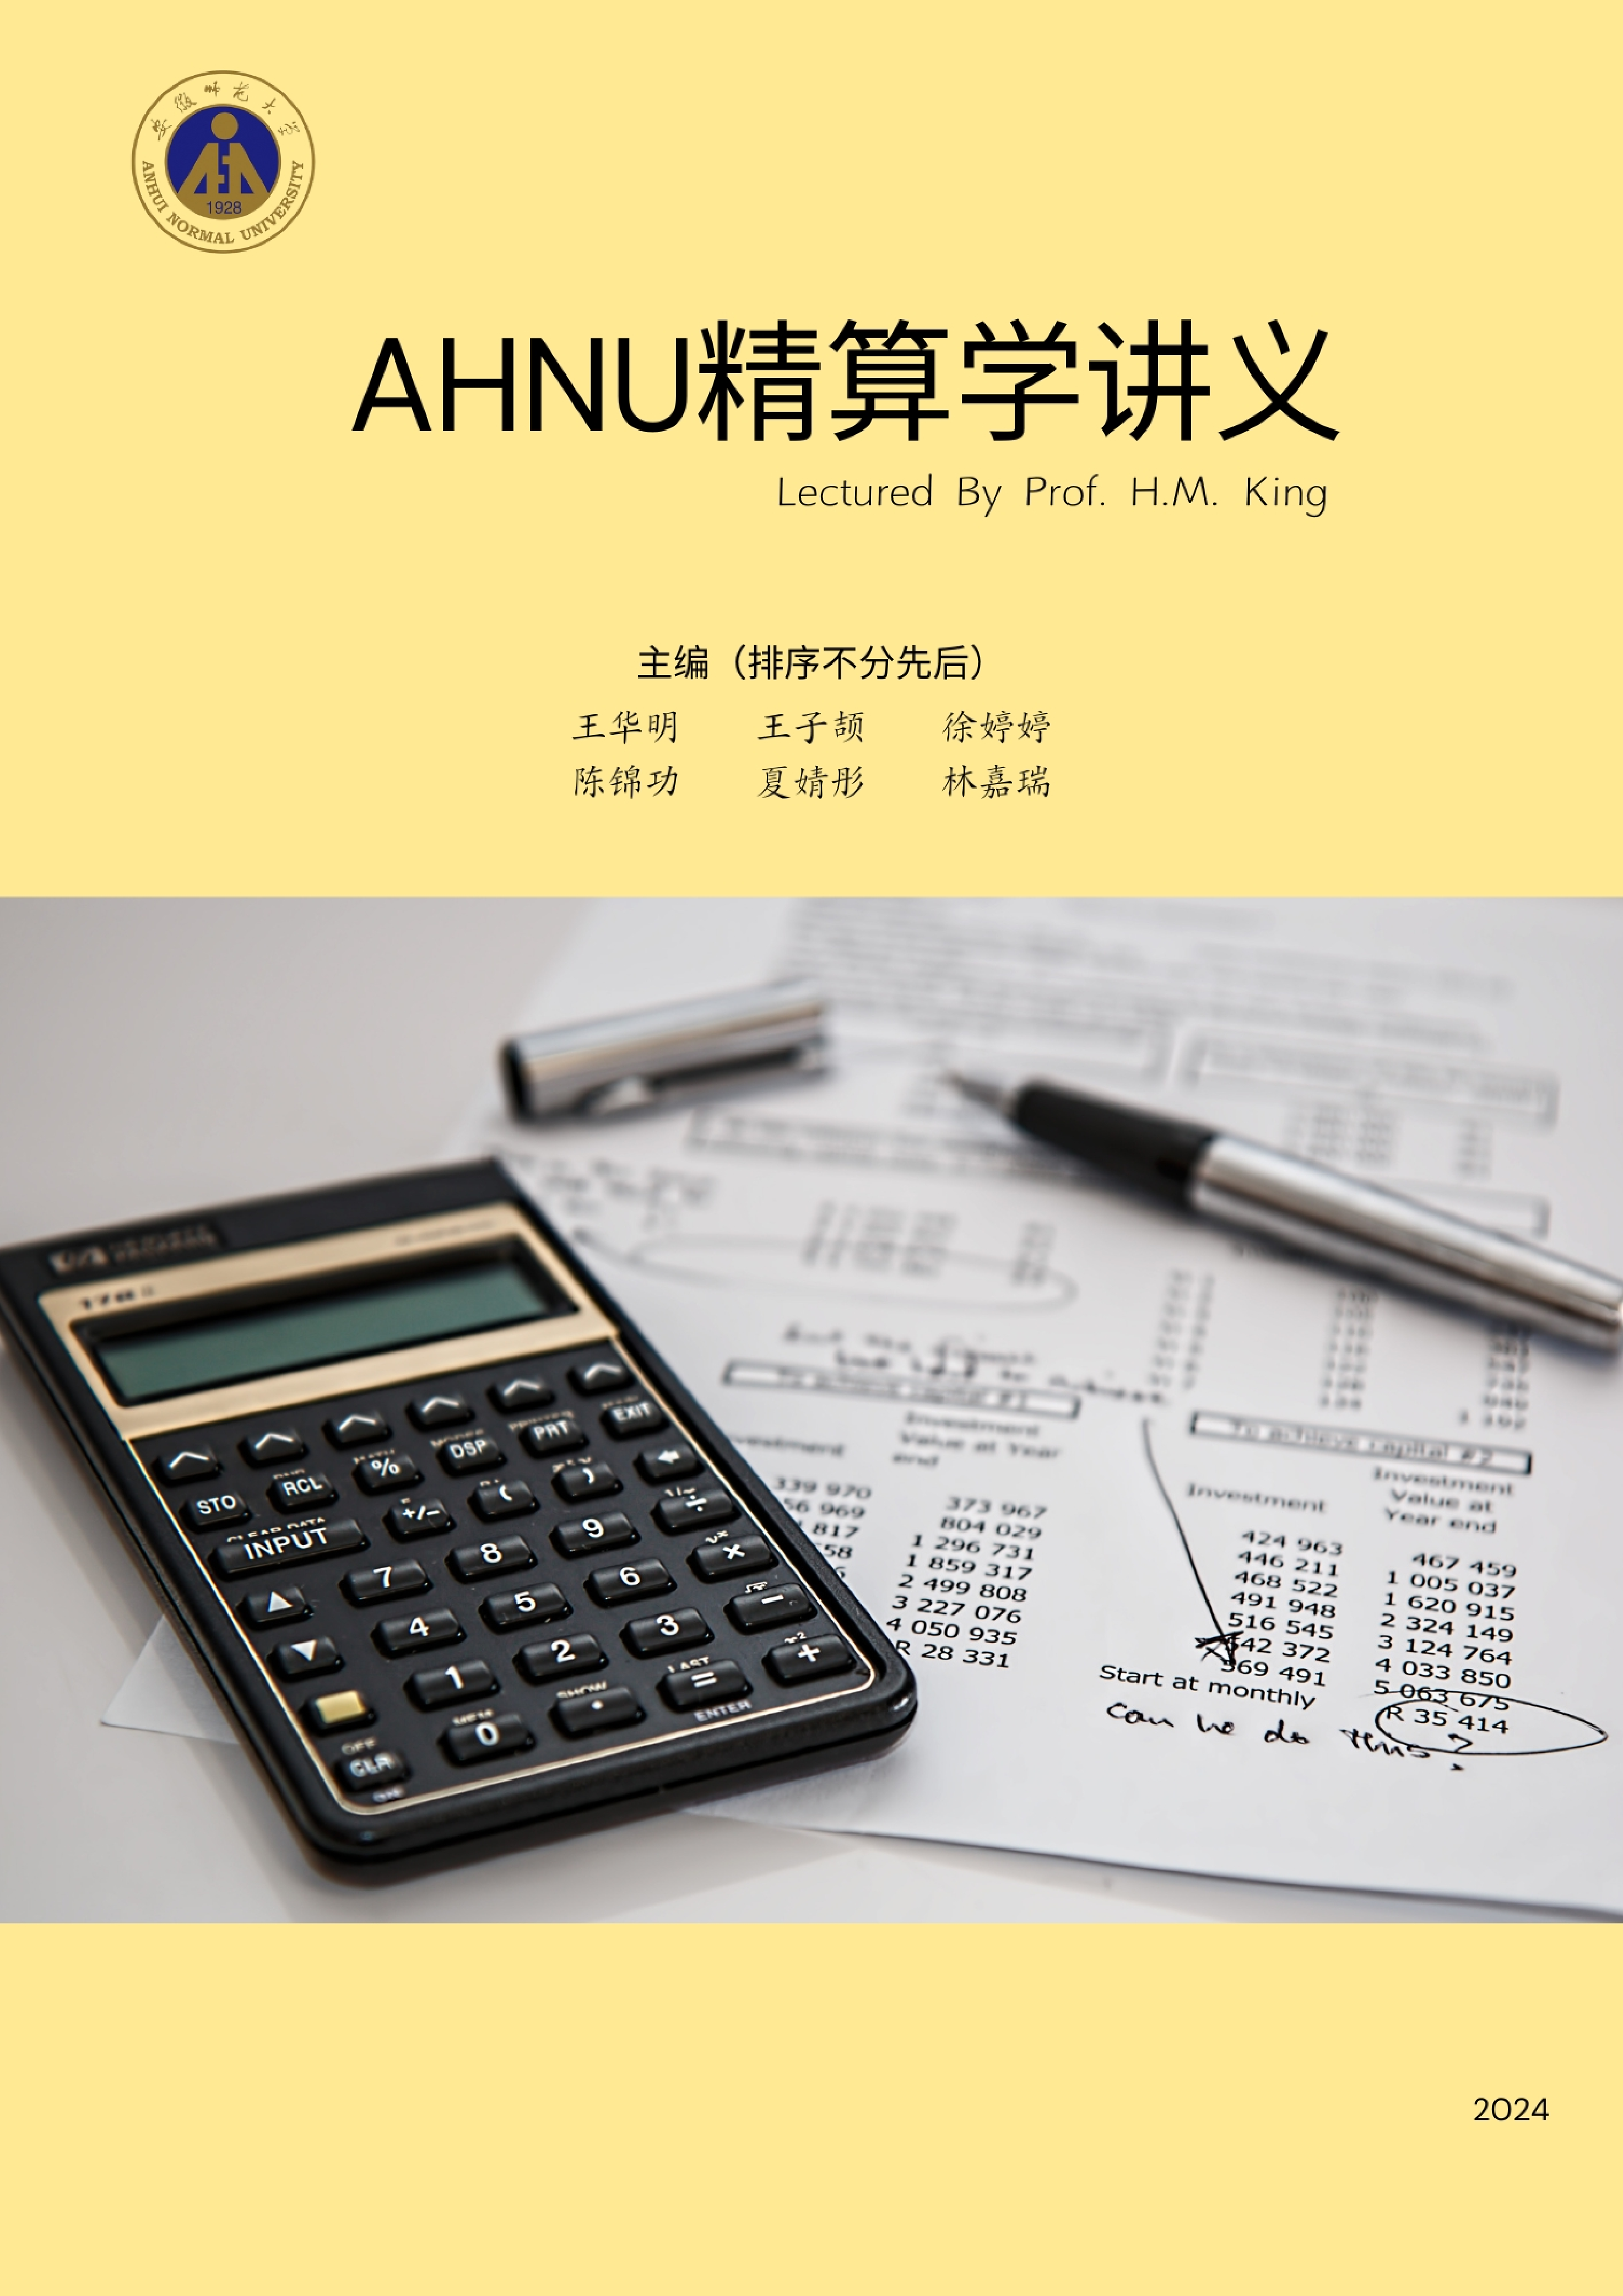
\includepdf{PDFCover.pdf}

%\large
\title{\Huge\textbf{《精算学》讲义}\footnote{本讲义由陈锦功、王子颉、林嘉瑞、夏婧彤、徐婷婷等几名同学协助录入.}}

\author{王华明\thanks{安徽师范大学数学与统计学院, 安徽芜湖(241003).  Email:hmking@ahnu.edu.cn}}
\date{}
\frontmatter
\maketitle

\vspace{-6mm}

\large
\begin{center}
    \begin{minipage}[c]{12cm}
        \begin{center}\textbf{序}\quad \end{center}
        \vspace{-0em} \hspace{2em} 本讲义是王华明老师在2023-2024年第2学期讲授的《精算学》课程笔记的电子版. 授课对象包括安徽师范大学2021级统计学专业全体同学及少数几位跨专业选课的同学. 教材选用的是北京大学出版社的《寿险精算基础》一书, 该书的作者是杨静平教授. 在此对北京大学出版社及杨静平教授表示感谢.

    \end{minipage}
\end{center}

%\tableofcontents
%\newpage


%\newpage
%% \pagestyle{empty}
%\section*{更新日志}
%2024.2.28
%
%由H.M. King老师领导的编写组成立, 由WZJ和LJR完成了初步模板的编写.
\newpage

\begin{center}
    {\bf\hei 精算学内容}
\end{center}
\begin{enumerate}
    \item 你能活多久?(生存分布)
    \item 你死的时候, 保险公司支付你1元, 这1元的现值为多少?(人寿保险)
    \item 在你活着时, 保险公司每年支付你1元, 这些支付的现值是多少?(生存年金)
    \item 上述的寿险与生存年金, 你该向保险公式缴纳多少保费?(保费理论)
    \item 保险公司为了保证支付, 要准备多少钱?(准备金理论)
\end{enumerate}
\newpage
\thispagestyle{empty}

\mainmatter
\chapter{生存分布}
\section{新生儿的生存分布}
\begin{itemize}
    \item[{\bf\hei 一.}]{\bf\hei 生存函数}
\end{itemize}

设有一个新生儿, 其寿命记为$X,$ 则$X$是一个非负随机变量. 假设$X$为一个连续型随机变量, 其分布函数为$F_X(x),$ 密度函数为$f_X(x).$ 回忆一下, 我们有 $F_X(x)=\int_0^x f_X(t)dt$ 且在$f_X(x)$的连续点上有
$$F_X'(x)=f_X(x).$$
如下我们总假设密度函数$f_X(t)$连续.
\begin{definition}
    称$s(t):=P(X>t),t>0$ 为$X$的生存函数.
\end{definition}
易知
\begin{align}\label{sf}
    s(t)=1-F_X(t), s'(t)=-f_X(t).
\end{align}

\begin{itemize}
    \item[{\bf\hei  二.}]{\bf\hei 死亡力}
\end{itemize}

现欲刻画一个$t$时刻还活着的个体瞬间死去的可能性, 做如下计算:

\begin{align}\label{swl}
    \lim_{h\downarrow0} & \frac{P(t<X\le t+h|X>t)}{h}=\lim_{h\downarrow0} \frac{P(t<X\le t+h)}{hP(X>t)}\no                                            \\
                        & =\lim_{h\downarrow0}\frac{P(X\le t+h)-P(X\le t)}{hP(X>t)}=\lim_{h\downarrow0}\frac{F_X(t+h)-F_X(t)}{h}\frac{1}{1-F_X(t)}\no \\
                        & =\frac{F_X'(t)}{1-F_X(t)}=\frac{f_X(t)}{1-F_X(t)}=-\frac{s'(t)}{s(t)}.
\end{align}

\begin{definition}
    称$\mu(t):=-\frac{s'(t)}{s(t)},t\ge 0$ 为新生儿的死亡力函数.
\end{definition}
由\eqref{swl}中的计算可知, 死亡力$\mu(t)$刻画了新生儿在$t$附近死去的``快慢".

\begin{proposition} 关于$\mu(t),$ $s(t)$ 及 $f_X(t)$ 有如下结论:

    {\rm\bf(i)} $\mu(t)=-\frac{s'(t)}{s(t)}=\frac{f_X(t)}{1-F_X(t)}=\frac{f_X(t)}{s(t)};$

    {\rm\bf(ii)} $f_X(t)=\mu(t)s(t);$

    {\rm\bf(iii)} $s(t)=e^{-\int_0^t\mu(s)ds}.$

\end{proposition}
\proof (i)和(ii)可由死亡力$\mu(t)$的定义及(1)式直接得出. 现证明(iii). 注意到$s(0)=P(X>0)=1$及
$$\mu(t)=-\frac{s'(t)}{s(t)}=-[\ln s(t)]'.$$ 所以有
$$\ln s(t)=-\int_0^t\mu(s)ds.$$ 故$s(t)=e^{-\int_0^t\mu(s)ds},$ (iii) 得证. \qed


\begin{remark}
    \begin{enumerate}
        \item[{\bf(a)}] 由$s(t) = e^{-\int_{0}^{t}\mu(s)\mathrm{d}s}$及$ \mu(t) = -\frac{s'(t)}{s(t)}$ 可知, 生存函数$s(t)$ 与死亡力函数$\mu(t)$ 相互唯一确定.
        \item[{\bf(b)}] 一个函数$\mu(t)$要作为死亡力, 必须满足以下两条:
            \begin{enumerate}
                \item[ $ 1^\circ$] $\mu(t) \geq 0, ~\forall t \geq 0$ (保证$s(t)$单调递减).
                \item[$2^\circ$] $\int_0^{\infty}\mu(t)\mathrm{d}t = \infty$(保证$s(\infty)=0$).
            \end{enumerate}
    \end{enumerate}

\end{remark}




\begin{example}
    假设新生儿的寿命服从以$\lambda$为参数的指数分布, 则密度函数$f_X(t)=\lambda e^{-\lambda x},x>0.$ 分布函数$F_X(t)=\int_0^t f_X(s)ds=1-e^{-\lambda t}, t>0.$ 生存函数$s(t)=1-F_X(t)=e^{-\lambda t},t>0.$  故其死亡力函数为
    \begin{align}\label{ep}
        \mu(t)=-\frac{s'(t)}{s(t)}=-\frac{-\lambda e^{-\lambda t}}{e^{\lambda t}}\equiv\lambda.
    \end{align}
\end{example}

\begin{remark}
    由\eqref{ep}式可知, 若新生儿寿命服从以$\lambda$ 为参数的指数分布, 则死亡力$\mu(t)\equiv \lambda,$ 和$t$无关. 这表示新生儿的死亡力在任何时候都是一样的. 也就是说, 新生儿永远年轻. 这当然与实际情况不符. 所以, 指数分布作为寿命分布是有缺陷的. 但由于指数分布的计算较为简单, 所以在理论研究中, 学者们很多时候都采用指数分布作为寿命分布.
\end{remark}
\begin{itemize}
    \item[{\bf\hei 三.}]{\hei\bf 整数年龄与分数年龄}
\end{itemize}
很多时候, 保险金都是在整数时刻支付的. 所以有必要研究整数年龄和分数年龄. 设$K(0)$为$X$的整数部分, $S(0)$为$X$的分数部分. 即
$$X = K(0) + S(0).$$
记$\mathring{e}_0 = E(X),$ 它表示新生儿的期望寿命; 记$e_0 = E(K(0)),$ 它表示期望整数寿命. 易知
\begin{equation*}
    e_0 \le \mathring{e}_0 < e_0 + 1.
\end{equation*}

\begin{lemma}\label{lemm0}
    设随机变量$X$的$n$阶矩存在, 即$E(X^n) < \infty,$ 则$\lim_{M \rightarrow \infty}M^ns(M) = 0.$
\end{lemma}
\begin{proof} 注意到
    \begin{align}
        E(X^n)=\int_{0}^\infty s^n f_X(s)ds=\int_0^Ms^n f_X(s)ds +\int_{M}^\infty s^n f_X(s)ds.
    \end{align}
    因$X$的$n$阶矩存在, 故上式左右两端都是有限的. 由于 $\lim_{M\rto} \int_0^Ms^n f_X(s)ds=E(X^n),$ 所以
    $\lim_{M\rto}\int_{M}^{\infty} s^nf_X(s)\mathrm{d}s=0.$ 于是
    \begin{align}
        M^n s(M) & = M^nP(X>M)
        =    \int_{M}^{\infty} M^nf_X(s)\mathrm{d}s  \no                                 \\
                 & \leq \int_{M}^{\infty} s^nf_X(s)\mathrm{d}s \rightarrow 0,\ M\rto.\no
    \end{align}
    引理证毕. \qed
\end{proof}

\begin{proposition}如下结论成立:
    \begin{enumerate}
        \item[(1)] $\mathring{e}_0 = E(X) = \int_0^{\infty}s(t)\mathrm{d}t;$
        \item[(2)] $E(X^2) = \int_{0}^{\infty} 2ts(t)\mathrm{d}t;$
        \item[(3)] $E(K(0)^2) = \sum_{n = 1}^{\infty} (2n-1)s(n);$
        \item[(4)] $e_0=E(K(0)) = \sum_{n = 1}^{\infty} s(n).$
    \end{enumerate}
\end{proposition}
\begin{proof}由分部积分公式和引理\ref{lemm0}可知
    \begin{equation*}
        \begin{aligned}
            {E}\left(X^{n}\right) & =\int_0^\infty t^n\mathrm{d}F(t)=\lim_{M\to\infty}\int_0^Mt^n\mathrm{d}F(t)=-\lim_{M\to\infty}\int_0^Mt^n\mathrm{d}s(t) \\
                                  & \left.=-\lim_{M\to\infty}(\left[t^ns(t)\right]\right|_0^M-\int_0^Mnt^{n-1}s(t)\mathrm{d}t)                              \\
                                  & =\lim_{M\to\infty}[-M^ns(M)]+\lim_{M\to\infty}\int_0^Mnt^{n-1}s(t)\mathrm{d}t                                           \\
                                  & =\int_0^\infty nt^{n-1}s(t)\mathrm{d}t.
        \end{aligned}
    \end{equation*}
    故(1)与(2)得证. 下证(3), 由离散型随机变量函数期望的计算公式, 有
    \begin{align*}
        E(K(0)^2) & = \sum_{k = 0}^{\infty} k^2P(K(0) = k)
        = \sum_{k = 0}^{\infty} k^2[P(X \geq k) - P(X \geq k+1)]                                                            \\
                  & = \sum_{k = 0}^{\infty} k^2s(k) - \sum_{k = 0}^{\infty} k^2s(k+1)                                       \\
                  & =\sum_{k = 0}^{\infty} k^2s(k) - \sum_{k = 0}^{\infty} (k+1)^2s(k+1)+\sum_{k = 0}^{\infty} (2k+1)s(k+1) \\
                  & = \sum_{k = 0}^{\infty} (2k+1)s(k+1)                              = \sum_{n = 1}^{\infty} (2n-1)s(n).
    \end{align*}
    故(3)得证. 类似可证(4). \qed
\end{proof}

\section{$x$岁个体的生存分布}

\begin{itemize}
    \item[{\bf\hei 一.}]{\bf\hei $x$岁个体余命的分布、密度及生存函数}
\end{itemize}

为了方便, 今后将一个$x$岁还活着的个体记为$(x).$ 个体$(x)$的余命记为$T(x).$ 显然有
$$T(x)=X-x.$$
这里特别强调一下,
$T(x)$的分布表示在已知事件$\{X>x\}$发生的条件下, $X-x$的分布. 如果新生儿在$x$岁之前死了, 也就没有了所谓的个体$(x),$ 其余命也就无从谈起.

记$F_{T(x)}(t)$为$T(x)$的分布函数, 则
\begin{align}\label{ft}
    F_{T(x)}(t) & = P(T(x) \leq t|X > x)
    = P(X- x \leq t | X > x)\no                        \\
                & = \frac{P(x<X \leq t + x)}{P(X > x)}
    = \frac{P(X > x) - P(X > x + t)}{P(X > x)}\no      \\
                & = 1 - \frac{s(x+t)}{s(x)}.
\end{align}
记$f_{T(x)}(t)$为$T(x)$的密度函数, 则
\begin{equation}\label{ftd}
    f_{T(x)}(t) = F_{T(x)}'(t) = -\frac{s'(x+t)}{s(x)} = \frac{f_X(x+t)}{s(x)}.
\end{equation}
\begin{definition}
    称$s_{T(x)}(t): = P(T(x)>t)$为个体 $(x)$的的生存函数.
\end{definition}

由\eqref{ft}可得
\begin{align}\label{stf}
    s_{T(x)}(t)=1-F_{T(x)}(t)=\frac{s(x+t)}{s(x)} \text{ 且 }\  s_{T(x)}'(t)=-f_{T(x)}(t).
\end{align}


\begin{itemize}
    \item[{\bf\hei 二.}]{\bf\hei $x$岁个体的死亡力}
\end{itemize}
为了解个体$(x)$在$x+t$岁附近死去的``快慢", 考虑极限

\begin{align*}
    \lim_{\Delta t\to0+} & \frac{P(t<T(x)\leqslant t+\Delta t|T(x)>t)}{\Delta t}
    =  \lim_{\Delta t\to0+}\frac{P(t<T(x)\leqslant t+\Delta t)}{\Delta tP(T(x)>t)}                                          \\
                         & = \lim_{\Delta t\to0+}\frac{s_{T(x)}(t) - s_{T(x)}(t + \Delta t)}{\Delta t}\frac{1}{s_{T(x)}(t)}
    = - \frac{s_{T(x)}'(t)}{s_{T(x)}(t)}                                                                                    \\
                         & = - \frac{\frac{s'(x+t)}{s(x)}}{\frac{s(x+t)}{s(x)}}
    =  -\frac{s'(x+t)}{s(x+t)} = \mu(x+t).
\end{align*}

\begin{definition}
    称$\mu_x(t) = -\frac{s_{T(x)}'(t)}{s_{T(x)}(t)}$为$X$岁个体在$t$ 年后的死亡力函数.
\end{definition}

\begin{proposition}\label{p21} 我们有

    {\bf(i)} $s_{T(x)}(t)=1-F_{T(x)}(t)=\frac{s(x+t)}{s(x)};$

    {\bf(ii)} $\mu_{x}(t)=\frac{f_{T(x)}(t)}{1-F_{T(x)}(t)}=\frac{f_{T(x)}(t)}{s_{T(x)}(t)}=-\frac{s_{T(x)}'(t)}{s_{T(x)}(t)}.$

    {\bf(iii)} $f_{T(x)}(t)=s_{T(x)}(t)\mu_{x}(t);$

    {\bf(iv)} $\mu_x(t)=\mu(x+t);$

    {\bf(v)} $s_{T(x)}(t)=e^{-\int_0^t \mu_x(s)ds}=e^{-\int_0^t \mu(x+s)ds}=e^{-\int_x^{x+t} \mu(s)ds}.$

\end{proposition}
\proof 利用\eqref{ft}, \eqref{ftd} 和 \eqref{stf}, 很容易证明 (i), (ii), (iii). 下证(iv). 由(ii), \eqref{ftd} 及\eqref{stf} 可得,
\begin{align*}
    \mu_{x}(t)=\frac{f_{T(x)}(t)}{s_{T(x)}(t)}=\frac{f_{X}(x+t)/s(x)}{s(x+t)/s(x)}=\frac{f_{X}(x+t)}{s(x+t)}=\mu(x+t).
\end{align*}
其中, 为了得到最后一个等号, 我们用了命题1.1中的第一条. (iv)得证.

最后证明(v). 注意到$s_{T(x)}(0)=P(T(x)>0)=1$ 且由第(ii)条有
$$\mu_{x}(t)=-\frac{s_{T(x)}'(t)}{s_{T(x)}(t)}=-[\ln s_{T(x)}(t)]'.$$
故 $\ln s_{T(x)}(t)=-\int_0^t\mu_x(s)ds.$ 从而
$s_{T(x)}(t)=e^{-\int_0^t\mu_x(s)ds}.$ 又因为$\mu_x(t)=\mu(x+t),$ 故
\begin{align*}
    s_{T(x)}(t)=e^{-\int_0^t\mu_x(s)ds}=e^{-\int_0^t\mu(x+s)ds}=e^{-\int_x^{x+t} \mu(s)ds},
\end{align*}
其中, 为得到最后一个等号, 我们用定积分的换元法即可. \qed


\begin{remark}
    理论上, 一个人一旦出生, 其死亡力就``注定"了. 如果他在$x$岁还活着, 在$t$ 年后他变为$x+t$ 岁, 此时他的死亡力是$\mu_x(t).$ 换一种观点, 如果站在0 时刻(他出生时)看, 他在$x+t$岁的死亡力应为$\mu(x+t).$ 故有
    $$\mu_x(t)=\mu(x+t).$$
\end{remark}

\begin{example}
    设新生儿的寿命服从以$\lambda>0$ 为参数的指数分布. 则
    $s(t)=e^{-\lambda t}, t>0.$ 从而有
    \begin{align*}
         & F_{T(x)}(t)=1-\frac{s(x+t)}{s(x)}=1-\frac{e^{-\lambda(x+t)}}{e^{-\lambda x}}=1-e^{-\lambda t} =F_X(t); \\
         & f_{T(x)}(t)=F_{T(x)}'(t)=F_X'(t)=f_X(t);                                                               \\
         & \mu_x(t)=\mu(x+t)\equiv\lambda.
    \end{align*}
    以上计算再次表明, 在指数分布寿命假设下, 新生儿的的寿命$X$与$x$岁的个体的余命$T(x)$的分布相同. 进一步说明指数分布作为寿命分布是有缺陷的.
\end{example}


\begin{proposition}$\forall u,t>0,$ 有
    \begin{align}
         & P(T(x)>t+u|T(x)>t)=P(T(x+t)>u).\label{tu}
    \end{align}
    该式的含义为: 一个$x$岁的人, 在$x+t$岁还活着的条件下, 再活$u$年不死的概率与一个$x+t$岁的人再$u$年内未死的概率相等.
\end{proposition}

\proof 对$u,t>0,$ 由条件概率定义知
\begin{align*}
    P(T(x) & >t+u|T(x)>t)=\frac{P(T(x)>t+u)}{P(T(x)>t)}=\frac{P((X-x)>t+u)}{P((X-x)>t)} \\
           & =\frac{P(X-(x+t)>u)}{P(X>x+t)}=  P(X-(x+t)>u|X>x+t)                        \\
           & =P(T(x+t)>u)=\frac{P(T(x)>t+u)}{P(T(x)>t)}.
\end{align*}
命题证毕. \qed

\begin{remark}由\eqref{tu}式立即可得
    \begin{align}\label{tul}
         & P(T(x)\leq t+u|T(x)>t)=P(T(x+t)\leq u).
    \end{align}
\end{remark}
\begin{example}
    设新生儿的寿命服从指数分布, 参数为$\lambda$, 则$\mu(t)\equiv\lambda,$
    \begin{align*}
         & s(t)=e^{-\lambda t},t>0.                                                                                       \\
         & F_{T(x)}=1-\frac{s(x+t)}{s(x)}=1-e^{- \lambda t}=F_x(t).                                                       \\
         & f_{T(x)}(t)=F_{T(x)}(t)=\lambda e^{- \lambda t}=f_x(t),t>0.                                                    \\
         & s_{T(x)}(t)=\frac{s(x+t)}{s(x)}=e^{-\lambda t}=s(t),t>0.                                                       \\
         & \mu_x(t)=\mu(x+t)\equiv\mu,t>0.                                                                                \\
         & e_x = \sum_{k=1}^{\infty} {_kp_x}=\sum_{k=1}^{\infty} {e^{- \lambda t}}=\frac{e^{- \lambda}}{1-e^{- \lambda}}. \\
         & \mathring{e}_x=\int_{0}^{\infty}{_tp_x}dt=\int_{0}^{\infty}{e^{- \lambda t}}dt=\frac{1}{\lambda}.
    \end{align*}
    显而易见, 这里的$\mathring e_x $和$e_x$与$x$无关, 也就是说,  所有人的剩余寿命的期望都是一样的, 和他现在的年龄无关. 这进一步说明指数分布作为寿命分布是有缺陷的.   此外, 因$\mathring{e}_x=ET(x)=\frac{1}{\lambda},$ 故指数分布的参数$\lambda$正好是期望寿命的倒数.
\end{example}

\begin{itemize}
    \item[{\bf\hei 三.}]{\bf\hei 一些精算学表示法}
\end{itemize}
注意到 $ S_{T(x)}(t)=P(T(x)>t)$表示个体$ (x)$在$t$年后还活着的概率; 而$F_{T(x)}(t)=P(T(x)\le t)$表示个体$(x)$在$t$年内死去的概率. 这些记号都很复杂, 书写比较困难. 故精算学中需引入一些简单的记号.


定义如下几个记号:
\begin{enumerate}
    \item[$\mathring 1.$] 用$_tp_{x}\stackrel{\text{def}}{=}P(T(x)>t)=S_{T(x)}(t)$
        表示个体$(x)$在$t$年后还活着的概率. 显然有
        $$ {}_tP_x=S_{T(x)}(t)=\mathrm{e}^{-\int_{0}^{t}\mu_x(s)\mathrm{d}s}=\mathrm{e}^{-\int_{0}^{t}\mu(x+s)\mathrm{d}s}=\mathrm{e}^{-\int_{x}^{x+t}\mu(s)\mathrm{d}s}.$$
    \item[$\mathring 2.$] 用$_tq_{x}\stackrel{\text{def}}{=}P(T(x)\leq t)=F_{T(x)}(t)$
        表示一个$x$岁的人在$t$年内死亡的概率. 易知
        $$_tp_{x}+{}_tq_{x}=1.$$
    \item[$\mathring 3.$] 用$ _{u|t}q_x=P(u<T(x)\leq u+t)$
        表示一个$x$岁的人在$x+u$岁还活着, 但在未来$t$年内死亡的概率.
\end{enumerate}
\begin{proposition}如下几个结论成立:

    (i) $\frac{d(_tp_x)}{dt}=-_tp_x\mu_x(t);$

    (ii) $\frac{d(_tp_x)}{dx}= {}_tp_x(\mu(x)-\mu(x+t)).$


\end{proposition}

\proof (i) 注意到${}_tp_x=\mathrm{e}^{-\int_{0}^{t}\mu_x(s)ds}.$ 故
$$\frac{d(_tp_x)}{dt}=\frac{d(\mathrm{e}^{-\int_{0}^{t}\mu_x(s)ds})}{dt}=\mathrm{e}^{-\int_{0}^{t}\mu_x(s)ds}({-\int_{0}^{t}\mu_x(s)ds})^{\prime}_t=-_tp_x\mu_x(t).$$

(ii) 利用等式${}_tp_x=e^{-\int_{x}^{x+t}\mu_x(s)ds},$ 有
$$\frac{d(_tp_x)}{dx}=(e^{-\int_{x}^{x+t}\mu_x(s)ds})^{\prime}=e^{-\int_{x}^{x+t}\mu(s)ds}({-\int_{x}^{x+t}\mu(s)ds})^{\prime}_x= {}_tp_x(\mu(x)-\mu(x+t)).$$
命题证毕.
\qed

\begin{proposition}以下结论成立:

    (1) $f_{T(x)}(t)={}_tp_x\cdot \mu_x(t);$

    (2) $_tp_x={}_sp_x\cdot{}_{t-s}p_{x+s},0\leq s\leq t;$

    (3) ${}_{u|t}q_x={}_up_x-{}_{u+t}p_x, u,t>0;$

    (4) ${}_{u|t}q_x={}_up_x~{}_{t}q_{x+u},u,t\ge0.$
\end{proposition}
\proof (1)是显然的, 不需证明. (2)
固定$0\le s\le t,$ 则由条件概率性质可知
\begin{align*}
    {}_tp_x & =P(T(x)>t)=P(T(x)>s)P(T(x)>t|T(x)>s) \\
            & ={}_sp_xP(T(x)>t+s-s|T(x)>s)         \\
            & ={}_sp_xP(T(x+s)>t-s)                \\
            & ={}_sp_x\cdot{}_{t-s}p_{x+s}.\end{align*}

(3) 对$t,u\ge0,$ 简单计算可知
\begin{align*}
    {}_{u|t}q_x & =P(u<T(x)\leq u+t)                          \\
                & =P(T(x)>u)-P(T(x)>u+t)={}_up_x-{}_{u+t}p_x.
\end{align*}

(4) 固定$t,u\ge0,$ 利用\eqref{tul}得
\begin{align*}
    {}_{u|t}q_x & =P(u<T(x)\leq u+t)=P(T(x)>u)P(T(x)\leq u+t|T(x)>u) \\
                & ={}_up_xP(T(x+u)<t)= {}_up_x{}~_{t}q_{x+u}.
\end{align*}
命题证毕. \qed

\begin{itemize}
    \item[{\bf\hei 四.}]{\bf\hei 个体$(x)$的整数与分数余命}
\end{itemize}
类似处理新生儿的寿命一样, 可将个体$(x)$的余命$T(x)$分为整数部分和小数部分.
设
\begin{align*}
     & T(x)=K(x)+S(x)
\end{align*}
其中$K(x)$是$T(x)$的整数部分, $S(x)$是$T(x)$的小数部分. 记
\begin{align*}
     & \mathring{e}_x\stackrel{\text{def}}{=}E(T(x)), \   {e_x}\stackrel{\text{def}}{=}E(K(x))
\end{align*}
则简单计算可知 \begin{align*}
    \mathring{e}_x & =E(T(x))=\int_{0}^{\infty}P(T(x)>t)d t=\int_{0}^{\infty}{_tp_xdt};                          \\
    {e_x}          & =E(K(x))=\sum_{k=0}^{\infty}kP(K(x)=k)                                                      \\
                   & =\sum_{k=0}^{\infty}k[P(T(x)\geq k)-P(T(x)\geq k+1)]                                        \\
                   & =\sum_{k=0}^{\infty}k{}_kp_x-\sum_{k=0}^{\infty}k{}_{k+1}p_x=\sum_{k=0}^{\infty}{_{k+1}p_x} \\
                   & =\sum_{k=0}^{\infty}{_kp_x}.
\end{align*}

\section{随机生存群}
\begin{itemize}
    \item[{\bf\hei 一.}]{\bf\hei 模型描述}
\end{itemize}

设0时刻系统中有$l_0$个新生儿, 他们的寿命独立同分布, 服从某分布, 生存函数为$s(t),t\ge 0.$  记

$\mathscr{L}(x)$ 为在$x$ 岁还活着的总人数;

$_t \mathscr{D}_x$为$[x,x+t]$内死去的总人数.

设系统中初始时刻的$l_0$个人的寿命分别为$X_1,X_2,?,X_n$, 则他们独立同分布, 且
$$P(X_i>t)=s(t), i=1,...,n.$$
显然有
\begin{align*}
     & \mathscr{L}(x)=\sum_{i=1}^{\iota_{\mathrm{0}}}I_{\{X_{i}\geqslant x\}},\ {}_t\mathscr{D}_x=\sum_{i=1}^{l_0}I_{\{ x\leqslant X_i<x+t\}}
\end{align*}
其中
$
    I_{A}=\left\{\begin{array}{ll}1,&\omega\in A,\\0,&\omega\in A^c\end{array}\right.
$ 为示性函数.

令 \begin{align*}
    l_x     & \overset{def}{=}E\z(\mathscr L(x)\y), \text{ 它表示在}x\text{岁还活着的期望人数};         \\
    {}_td_x & \overset{def}{=}E\z({}_t\mathscr D_x \y),\text{ 它表示在}[x,x+t)\text{内死去人数的期望}.
\end{align*}



\begin{itemize}
    \item[{\bf\hei 二.}]{\bf\hei 几个结论}
\end{itemize}

\begin{proposition} 如下结论成立:
    $$l_x=l_0s(x),\ {}_td_x=l_x-l_{x+t}.$$
\end{proposition}
\proof 注意到$E(1_A)=P(A),$ 所以
\begin{align*}
    l_x     & =E(\mathscr{L}(x))=E(\sum_{k=1}^{l_0}I_{\{X_k>x\}})                        \\
            & =\sum_{k=1}^{l_0}E(I_{\{X_k>x\}})
    =\sum_{k=1}^{l_0}P(X_k>x)
    =\sum_{k=1}^{l_0}P(X_1>x)                                                            \\
            & =l_0P(X_1>x)=l_0s(x);                                                      \\
    {}_td_x & =E(_t\mathscr{D}_t)=E(\sum_{k=1}^{l_0}I_{\{x<X_k\leq x+t\}})               \\
            & =\sum_{k=1}^{l_0}E(I_{\{x<X_k\leq x+t\}})=\sum_{k=1}^{l_0}P(x<X_k\leq x+t) \\
            & =l_0P(x<X_1\leq x+t)=l_0[P(X_1>x)-P(X_1>x+t)]                              \\
            & =l_0s(x)-l_0s(x+t)
    =l_x-l_{x+t}.
\end{align*}

引入$l_x$及${}_td_x$的目的是为了计算生存概率${}_tp_x$与死亡概率${}_tq_x.$
\begin{proposition}如下结论成立:

    (i) ${}_tp_x=\frac{l_{x+t}}{l_x},$  ${}_tq_x=\frac{{}_td_x}{l_x},$  $l_{x+t}=l_xe^{-\int_{x}^{x+t}\mu(s)ds}$

    (ii) $\frac{dl_x}{dx}=-l_x\mu(x),$ $_nd_x=\int_{x}^{x+n}l_y\mu(y)dy.$
\end{proposition}

\proof 我们先证(i). 由$l_x=l_0s(x)$知$s(x)=\frac{l_x}{l_0}$, 所以
$$_tp_x=s_{T(x)}(t)=\frac{s(x+t)}{s(x)}=\frac{l_{x+t}/l_0}{l_x/l_0}=\frac{l_{x+t}}{l_x}.$$
由此可推出\begin{align*}
     & l_{x+t}=l_x\cdot{}_tp_x=l_xe^{-\int_{x}^{x+t}\mu(s)ds};                          \\
     & {}_tq_x=1-_tp_x=1-\frac{l_{x+t}}{l_x}=\frac{l_x-l_{x+t}}{l_x}=\frac{_td_x}{l_x}.
\end{align*}

下证(ii). 由(i)知,
$$\frac{dl_x}{dx}=l_0e^{-\int_{0}^{x}\mu(t)dt}(-\mu(x))=l_0s(x)(-\mu(x))=-l_x\mu(x).$$
由此可导出
$${}_nd_x=l_x-l_{x+n}=-\int_{x}^{x+n}\frac{d(l_y)}{dy}dy=\int_{x}^{x+n}l_y\mu(y)dy.$$
命题证毕.
\qed

补充:
$${}_td_x=\int_x^{x+t} l_yu(y)dy.$$

等式含义:左端表示在$[x,x+h]$内死去的人数, $u(y)dy=-\dfrac{s'(y)}{s(y)}dy=-\dfrac{d(s(y))}{s(y)}=\dfrac{s(y)-s(y+\Delta y)}{s(y)}.$所以$u(y)dy$表示一个人在$y$岁还活着的条件下,在$[y,y+dy]$ 内死去的概率,于是$l_yu(y)dy$表示在$[y,y+dy]$内死去的人数.对$y$积分(求和)可知$\int_x^{x+t}l_yu(y)dy$表示在$[x,x+t]$内死去的人数.

所以右端=左端.
\section{生命表的元素}
补充知识:

{\rm\bf(i)} 在精算学中, 若左下标是1,通常将其省略, 例如
$${p_x}\triangleq{}_1p_x,{q_x}\triangleq{}_1q_x,$$
$$L_x\triangleq{}_1L_x,{}_{u|}q_x\triangleq{}_{u|1}q_x.$$

{\rm\bf(ii)} $a\wedge b=\min\{a,b\},\ a\vee b=\max\{a,b\},\ EX=\int_0^{\infty}xf(x)dx,X\ge0.$

下面用两种方法计算$E(X\wedge t).$


法一:
\begin{align*}
    E(X\wedge t) & =\int_0^{\infty}(x\wedge t)f(x)dx                           \\
                 & =\int_0^t(x\wedge t)f(x)dx+\int_t^{\infty}(x\wedge t)f(x)dx \\
                 & =\int_0^txf(x)dx+\int_t^{\infty}tf(x)dx                     \\
                 & =\int_0^txf(x)dx+tP(X>t).
\end{align*}
\qed

法二:
\begin{align*}
    E(X\wedge t) & =E[(X\wedge t)I]                                \\
                 & =E((X\wedge t)[I_{x<t}+I_{x\ge t}])             \\
                 & =E((X\wedge t)I_{x<t})+E((X\wedge t)I_{x\ge t}) \\
                 & =E(XI_{x<t})+E(tI_{x\ge t})                     \\
                 & =\int_0^{\infty}xI_{x<t}f(x)dx+tE(I_{x\ge t})   \\
                 & =\int_0^t xf(x)dx+tP(X\ge t).                   \\
\end{align*}
\qed

{\rm\bf(iii)} 条件数学期望. 设$A$是一个随机事件, $X$为一个随机变量, 给定事件$A$的条件下, $X$的条件期望定义为

$$E(X|A)\overset{def}{=}\frac{E(XI_A)}{EI_A}=\frac{E(XI_A)}{P(A)}.$$


\begin{itemize}
    \item[{\bf\hei 一.}]{\bf\hei ${}_tL_x:$ 所有人在$[x,x+t)$内活过的总时间}
\end{itemize}


一个体$(x)$在$[x,x+t)$内活过的总时间为$T(x)\wedge t$, 这是因为

若$T(x)<t$, 则$(x)$在$[x,x+t)$内活过的时间$T(x).$

若$T(x)\ge t$, 则$(x)$在$[x,x+t)$内活过的时间$t.$

又因为在$x$还活着的人有$l_x$个, 故所有人在$[x,x+t)$内活的总时间为$l_x(T(x)\wedge t)$, 记其期望为$$ {}_tL_x=l_xE(T(x)\wedge t).$$

\begin{proposition} 如下结论成立:
    \begin{align*}
        {}_tL_x & =l_xE(T(x)\wedge t)                 \\
                & =\int_0^t sl_{x+s}u(x+s)ds+tl_{x+t} \\
                & =\int_0^tl_{x+s}ds
    \end{align*}
\end{proposition}
\proof 第一个等式是定义. 现证第二个等式. 注意到
\begin{align*}
    {}_tL_x & =l_xE(T(x)\wedge t)                                                                  \\
            & =l_x\int_0^{\infty} (s\wedge t){}_sp_x\mu_x(s)ds                                     \\
            & =\int_0^{\infty}(s\wedge t)l_{x+s}\mu(x+s)ds                                         \\
            & =\int_0^tsl_{x+s}\mu(x+s)ds+\int_t^{\infty}tl_{x+s}\mu(x+s)ds                        \\
            & =\int_0^tsl_{x+s}\mu(x+s)ds+tl_{x+t}\int_t^{\infty}\frac{l_{x+s}}{l_{x+t}}\mu(x+s)ds
\end{align*}

其中,\begin{align*}
    \int_t^{\infty}\frac{l_{x+s}}{l_{x+t}}\mu(x+s)ds
     & =\int_0^{\infty}\frac{l_{x+t+u}}{l_{x+t}}\mu(x+t+u)du \\
     & =\int_0^{\infty}{}_up_{x+t}\mu_{x+t}(u)du             \\
     & =\int_0^{\infty}f_{T{(x+t)}}(u)du                     \\
     & =1.
\end{align*}

于是 , ${}_tL_x=\int_0^tsl_{x+s}\mu(x+s)ds+tl_{x+t}.$ 故第二个等式成立.


下证第三个等式. 注意到
$$dl_y=-l_y\mu(y)dy$$
$$\Rightarrow dl_{x+s}=-l_{x+s}\mu(x+s)ds$$
$$\Rightarrow\int_0^tsdl_{x+s}=-\int_0^tsl_{x+s}\mu(x+s)ds.$$
由此可知$$sl_{x+s}\vert^{t}_{0}-\int_0^tl_{x+s}ds=-\int_0^tsl_{x+s}\mu(x+s)ds.$$
所以
$$\int_0^tsl_{x+s}\mu(x+s)ds+tl_{x+t}=\int_0^tl_{x+s}ds.$$
第三个等式得证.
\qed

表达式$\int_0^tsl_{x+s}\mu(x+s)ds+tl_{x+t}$的含义如下:

\noindent 一方面, 在$x+s$岁活着的人有$l_{x+s}$个, 每个人在$[x+s,x+s+ds]$内死去的概率为$\mu(x+s)ds,$ 所以, 在$[x+s,x+s+ds]$内死去的人数为$l_{x+s}\mu(x+s)ds$, 他们每个人在$[x,x+t]$内活$s$年, 所以在$x+s$岁死去的人在$[x,x+t]$内活的总时间为$sl_{x+s}\mu(x+s)ds,$ 再对$s$在$(0,t)$求积分(求和)可知, $\int_0^tsl_{x+s}\mu(x+s)ds+tl_{x+t}$表示在$[x,x+t]$内死去的人在这段时间内活过的总时间. 另一方面在$x+t$ 岁还活着的人有$l_{x+t},$ 每个人在$[x,x+t)$内活了$t$岁, 他们在$[x,x+t)$内总共活了$tl_{x+t}$岁.

综合以上分析, $\int_0^tsl_{x+s}\mu(x+s)ds+tl_{x+t}$表示所有人在$[x,x+t]$内活过的总时间, 这是一个复杂的公式, 但它有一个简单的表达$\int_0^tl_{x+s}ds.$

\begin{itemize}
    \item[{\bf\hei 二.}]{\bf\hei $a(x):$ 一个$x$岁的人在1年内死去的条件下, 在$[x,x+t)$内活过的期望时间}
\end{itemize}

个体$(x)$的余命为$T(x)$, 所以$$a(x)=E(T(x)|T(x)\le1).$$
\begin{proposition}以下等式成立:
    $$a(x)=\dfrac {\int_0^1t{}_tp_xu_x(t)dt}{q_x}.$$
\end{proposition}
\proof 利用条件数学期望的定义得
\begin{align*}
    a(x) & =E(T(x)|T(x)\le1)                                                \\
         & =\dfrac {E(T(x)I_{\{T(x)\le1\}})}{P(T(x)\le1)}                   \\
         & =\dfrac {\int_0^{\infty}tI_{\{T(x)\le1\}}f_{T(x)}(t)dt}{q_x}     \\
         & =\dfrac {\int_0^{\infty}tI_{\{T(x)\le1\}}{}_tp_x\mu_x(t)dt}{q_x} \\
         & =\dfrac {\int_0^1t{}_tp_x\mu_x(t)dt}{q_x}.
\end{align*}
命题证毕.\qed

利用$a(x)$可以给出$L_x$的另一个表达式.
\begin{proposition}如下
    等式成立: $$L_x=d_xa(x)+l_{x+1}.$$
\end{proposition}
\proof 由$L_x$的定义可知
\begin{align*}
    L_x & =l_xE(T(x)\wedge1)                                                     \\
        & =l_xE(T(x)\wedge1)I_{\{T(x)<1\}})+l_xE(T(x)\wedge 1)I_{\{T(x)\ge 1\}}) \\
        & =l_xE(T(x)*I_{\{T(x)<1\}})+l_xE(1*I_{\{T(x)\ge 1}\})                   \\
        & =l_xP(T(x)<1)E(T(x)|T(x)<1)+l_xP(T(x)\ge 1)                            \\
        & =l_xq_xa(x)+l_xp_x                                                     \\
        & =d_xa(x)+l_{x+1}.
\end{align*}
证毕. \qed

表达式$L_x=d_xa(x)+l_{x+1}$的含义如下:

\noindent 右端的$d_xa(x)$表示$[x,x+1)$内死去的人在$[x,x+1)$内活过的总时间. 右端的$l_{x+1}*1$表示在$x+1$岁活着的$l_{x+1}$人在$[x,x+1)$内活过的总时间, 所以右端表示所有人在$[x,x+1)$ 活过的总时间,等于左端的$L_x.$
\begin{itemize}
    \item[{\bf\hei 三.}]{\bf\hei ${}_nm_x=\dfrac {{}_nq_x}{\int_0^n{}_tp_xdt}$(中心死亡率)}
\end{itemize}


\begin{proposition}如下结论成立:
    $${}_nm_x=\dfrac{{}_nd_x}{{}_nL_x}.$$
\end{proposition}
\proof 简单计算可得
$${}_nm_x=\dfrac{{}_nq_x}{\int_0^n{}_tp_xdt}=\dfrac{{}_nd_x/l_x}{\int_0^n\dfrac{l_{x+t}}{l_x}dt}=
    \dfrac{{}_nd_x}{{}_nL_x}.$$命题证毕.\qed

\begin{itemize}
    \item[{\bf\hei 四.}]{\bf\hei $T_x\triangleq\int_0^{\infty}l_{x+s}ds={}_{\infty}L_x$}
\end{itemize}
显而易见, 表示所有人在$[x,\infty)$内活过的总时间.

\begin{itemize}
    \item[{\bf\hei 五.}]{\bf\hei $Y_x\triangleq\int_0^{\infty}T_{x+s}ds$}
\end{itemize}

生命表中包含$q_x,l_x,d_x,L_x,T_x,\mathring{e}_0$等元素. 总的来说, 利用生命表可以计算出生存概率${}_kp_x,$ 死亡概率${}_kq_x$、${}_{k|j}q_x$等.
\newpage

\section{分数年龄上的死亡假设}
\begin{itemize}
    \item[{\bf\hei 一.}]{\bf\hei 为什么引入分数年龄死亡力假设?}
\end{itemize}

$_{k}P_{x}=\frac{l_{x+k}}{l_{x}},$若$k$为整数, 可查生命表计算$_{k}P_{x},$例如: $_{2}P_{20}=\frac{l_{22}}{l_{20}}.$

但如果$k$不是整数, 例如: $_{2.5}P_{20}=\frac{l_{22.5}}{20},$求$l_{22.5}$的值. 发现无法查表得出.
则可以令$T(x)=K(x)+S(x),$其中K(x)是整数部分, S(x)是分数部分.

关于S(x)服从的分布可以满足以下两个假设:

{\rm\bf(i)}死亡力均匀分布假设$S(x)\sim U(0,1)$

{\rm\bf(ii)}常数死亡力假设.

\begin{itemize}
    \item[{\bf\hei 二.}]{\bf\hei 死亡力均匀分布假设(UDD假设)}
\end{itemize}

{\rm\bf(i)}定义: 若$x$为非负整数, $s(t)$是生存函数, 若$\forall t\in [0,1),$都有:
\begin{align}\label{tul}
     & s(x+t)=(1-t)s(x)+ts(x+1).
\end{align}

称在$[x,x+1)$上, 死亡力均匀分布假设成立.

{\rm\bf(ii)}设$[x,x+1)$上UDD假设成立, 则有以下结论:
\begin{enumerate}
    \item[$\mathring 1.$] $l_{x+t}=(1-t)l_{x}+tl_{x+1},t\in [0,1).$

        \proof \begin{align*}
            l_{x+t} & =l_{0}s(x+t)                 \\
                    & =l_{0}(1-t)s(x)+l_{0}ts(x+1) \\
                    & =(1-t)l_{x}+tl_{x+1}.
        \end{align*}
        证毕.\qed
    \item[$\mathring 2.$] $_{t}d_{x}=td_{x},t\in [0,1).$

        \proof \begin{align*}
            _{t}d_{x} & =l_{x}-l_{x+t}             \\
                      & =l_x-(1-t)l_{x}-tl_{x+t}   \\
                      & =t(l_{x}-l_{x+1}) =td_{x}.
        \end{align*}
        证毕.\qed
    \item[$\mathring 3.$] $_{t}q_{x}=tq_{x},t\in [0,1).$

        \proof \begin{align*}
            _{t}q_{x} & =\frac{_{t}d_{x}}{l_{x}} =\frac{td_{x}}{l_{x}}  = tq_{x}.
        \end{align*}
        证毕.\qed
    \item[$\mathring 4.$] $f_{T(x)}(t)=q_{x},t\in [0,1).$

        该结论可以反映均匀分布.

        \proof \begin{align*}
            f_{t(x)}(t) & =\frac{d(_{t}q_{x})}{dt} =\frac{d(tq_{x})}{dt} =q_x.
        \end{align*}
        证毕.\qed
    \item [$\mathring 5.$] $\mu_{x}(t)=\frac{q_{x}}{1-tq_x}$

          \proof \begin{align*}
              \mu_{x}(t) & =\frac{f_{t(x)(t)}}{S_{T(x)}(t)} =\frac{q_{x}}{_{t}p_{x}} =\frac{q_{x}}{1-_{t}q_{x}} =\frac{q_{x}}{1-tq_{x}}.
          \end{align*}
          证毕.\qed
\end{enumerate}

{\rm\bf(iii)}  \begin{proposition}已知在每一年龄年上UDD假设成立, 则$K(x)$与$S(x)$相互独立, 且$S(x)$服从$[0,1]$上的均匀分布.
\end{proposition}
\proof
考虑条件概率$P(S(x) \leq t \mid K(x) = k)$, 有
\begin{align*}
    P(S(x) \leq t \mid K(x) = k) & = \frac{P(S(x) \leq t, K(x) = k)}{P(K(x) = k)}                                                                          \\
                                 & = \frac{_{k|t}q_{x}}{_{k|}q_{x}} = \frac{_{k}p_{x}\,_{t}q_{x+k}}{_{k}q_{x}\,q_{x+k}} = \frac{_{t}q_{x+k}}{q_{x+k}} = t.
\end{align*}

因此, $K(x)$与$S(x)$相互独立, 且$S(x)$服从$[0,1]$上的均匀分布.

证毕.\qed

{\rm\bf(iv)}  \begin{proposition}在每一年龄年UDD假设成立时, 有
    $$\mathring{e}_{x}=e_{x}+\frac{1}{2}$$
    $$\text{Var}(T)=\text{Var}(K)+\frac{1}{12}$$
\end{proposition}
\proof
根据命题1.13的结果, 知$K(x)$与$S(x)$相互独立, 且$S(x)$服从$[0,1]$上的均匀分布, 因此有
\begin{align*}
    \mathring{e}_{x} & =E(K(x)+S(x))        \\
                     & = E(K(x))+E(S(x))    \\
                     & = e_{x}+\frac{1}{2}.
\end{align*}
及\begin{align*}
    \text{Var}(T(x)) & =\text{Var}(K(x)+S(x))             \\
                     & =\text{Var}(K(x))+\text{Var}(S(x)) \\
                     & =\text{Var}(K(x))+\frac{1}{12}.
\end{align*}
证毕.\qed

\begin{itemize}
    \item[{\bf\hei 三.}]{\bf\hei 常数死亡力假设}
\end{itemize}

{\rm\bf(i)}  定义: 设$x$为整数, 若$\forall t\in [0,1)$, 有
\begin{align}\label{tul}
    \ln s(x+t)=(1-t)\ln s(x)+t\ln s(x+1).
\end{align}
则称生存函数在年龄段$[x,x+1)$满足\textbf{常数死亡力假设}.

{\rm\bf(ii)}  \begin{proposition}设在年龄段$[x,x+1)$常数死亡力假设成立, 则对$t\in (0,1)$, 有
    \begin{enumerate}
        \item[$\mathring 1.$] 期望生存人数满足
            $$\ln l_{x+t}=(1-t)\ln l_{x}+t\ln l_{x+1};$$
            \proof 因$l_{x}=l_{0}s(x)$, 所以由公式(1.11), 知\begin{align*}
                \ln \frac{l_{x+t}}{l_{0}}=(1-t)\ln \frac{l_{x}}{l_{0}}+t\ln \frac{l_{x+1}}{l_{0}}.
            \end{align*}所以$\ln l_{x+t}=(1-t)\ln l_{x}+t\ln l_{x+1},$
            证毕.\qed
        \item[$\mathring 2.$] 死亡力为常数, 即
            $$\mu _{x}(t)=-\ln p_{x}\stackrel{\triangle}{=}\mu;$$
            \proof 对公式(1.11)取指数
            \begin{align*}
                                    & s(x+t)  =s(x)^{1-t}s(x+1)^{t}                              \\
                \Longleftrightarrow & {}_{x+t}p_{0} = {}_xp_{0}^{1-t}{}_{x+1}p_{0}^t             \\
                \Longleftrightarrow & {}_{x}p_{0}{}_{t}p_x = {}_xp_{0}~p_{x}^{t}                 \\
                \Longleftrightarrow & {}_{t}p_x = p_x^t                                          \\
                \Longleftrightarrow & e^{-\int_{0}^{t}\mu_x(s)ds} = e^{-\int_{0}^{t}-\ln p_x ds} \\
            \end{align*}
            可证$\mu _{x}(t)=-\ln p_{x}$.\qed
        \item[$\mathring 3.$] $$l_{x+t}=l_{x}e^{-\mu t},\ _{t}q_{x}=1-p^{t}_{x},\ f_{T(x)}(t)=-p_{x}^{t}\ln p_{x}.$$
            \proof \begin{align*}
                 & l_{x+t}=l_{x}e^{-\int_{x}^{x+t}\mu (s)ds}=l_{x}e^{-\mu t};         \\
                 & _{t}q_{x}=1-{}_{t}p_{x}=1-p_{x}^{t}=1-e^{t\ln p_{x}}=1-e^{-\mu t}; \\
                 & f_{T(x)}(t)={}_{t}p_{x}\mu {}_{x}(t)=p_{x}^{t}\mu=\mu e^{-\mu t}.
            \end{align*}.\qed
    \end{enumerate}
\end{proposition}

\begin{example}
    设$S(x)=1-\frac{x}{12},\ 0\leq x\leq 12$, $l_{0}$个个体相互独立, 生存函数都是$S(x)$.问:

    (1) 求$(_{3}\mathscr D _{0},\ _{3}\mathscr D_{3},\ _{3}\mathscr D _{6},\ _{3}\mathscr D _{9})$的联合分布;

    (2) 求这四个随机变量的期望和方差;

    (3) 求它们两两之间的相关系数.
\end{example}

\solution
易知$l_{0}$个人的寿命$X_{1},X_{2},...,X_{l_{0}}\stackrel{\text{i.i.d.}}{\sim}U[0,12]$.且随机变量满足
$$_{3}\mathscr D _{0}=\sum^{l_{0}}_{k=1}I_{\{0\leq x_k \leq 3\}}$$
$$_{3}\mathscr D _{3}=\sum^{l_{0}}_{k=1}I_{\{3\leq x_k \leq 6\}}$$
$$_{3}\mathscr D _{6}=\sum^{l_{0}}_{k=1}I_{\{6\leq x_k \leq 9\}}$$
$$_{3}\mathscr D _{9}=\sum^{l_{0}}_{k=1}I_{\{9\leq x_k \leq 12\}}$$

(1)令事件$A=\{_{3}\mathscr D _{0}=k_{1},\ _{3}\mathscr D _{3}=k_{2},\ _{3}\mathscr D _{6}=k_{3},\ _{3}\mathscr D _{9}=k_{4}\}$, 若事件$A$发生, 则认为在$l_{0}$中, 有$k_{1}$人在$[0,3]$死亡; 有$k_{2}$人在$[3,6]$死亡; 有$k_{3}$人在$[6,9]$死亡; 有$k_{4}$人在$[9,12]$死亡.其中$k_{1}+k_{2}+k_{3}+k_{4}=l_{0}.$从$k_{1}+k_{2}+k_{3}+k_{4}$个人中, 选出$k_{1}$个人在$[0,3]$内死亡, 有$C_{k_{1}+k_{2}+k_{3}+k_{4}}^{k_{1}}$种选法; 从$k_{2}+k_{3}+k_{4}$个人中, 选出$k_{2}$个人在$[3,6]$内死亡, 有$C_{k_{2}+k_{3}+k_{4}}^{k_{2}}$种选法; 从$k_{3}+k_{4}$个人中, 选出$k_{3}$个人在$[6,9]$内死亡, 有$C_{k_{3}+k_{4}}^{k_{3}}$种选法...以此推出:
$$
    P(A)=\frac{(k_{1}+k_{2}+k_{3}+k_{4})!}{k_{1}!k_{2}!k_{3}!k_{4}!}\cdot {}_{3}q_{0}^{k_{1}}\cdot {}_{3|3}q_{0}^{k_{2}}\cdot {}_{6|3}q_{0}^{k_{3}}\cdot {}_{9|3}q_{0}^{k_{4}}
$$

(2) 对于一个二项分布$B(n, p)$, 其期望$E[X] = np$, 方差$\text{Var}(X) = np(1-p)$.

因此, 对于每个随机变量$_{3}\mathscr D_{k}$:

期望: $$E(_{3}\mathscr D_{k}) = \frac{l_0}{4};$$

方差: $$\text{Var}(_{3}\mathscr D_{k}) = l_0 \cdot \frac{1}{4} \cdot \left(1 - \frac{1}{4}\right) = \frac{3l_0}{16}.$$

(3) 以$_{3}\mathscr D _{0},\ _{3}\mathscr D _{3}$的相关系数为例:
\begin{align*}
    \text{Cov}(_{3}\mathscr D _{0},\ _{3}\mathscr D _{3}) & =E(_{3}\mathscr D _{0}\ _{3}\mathscr D _{3})-E(_{3}\mathscr D _{0})E(_{3}\mathscr D _{3})                                \\
                                                          & =E(\sum ^{l_{0}}_{k=1}I_{\{0\leq x_{k}\leq 3\}}\cdot \sum ^{l_{0}}_{j=1}I_{\{3\leq x_{j}\leq 6\}})-(\frac{l_{0}}{4})^{2} \\
                                                          & =\sum^{l_{0}}_{k=1}\sum_{j\neq k}E(I_{\{0\leq x_{k}\leq 3\}}\cdot I_{\{3\leq x_{k}\leq 6\}})-(\frac{1}{4}l_{0})^{2}      \\
                                                          & =\frac{l_{0}(l_{0}-1)}{16}-\frac{l_{0}^{2}}{16}                                                                          \\
                                                          & =-\frac{l_{0}}{16}.
\end{align*}
(对于$\sum^{l_{0}}_{k=1}\sum_{j\neq k}E(I_{\{0\leq x_{k}\leq 3\}}\cdot I_{\{3\leq x_{k}\leq 6\}}) = \frac{l_{0}(l_{0}-1)}{16}$的理解: 其中$\sum^{l_{0}}_{k=1}\sum_{j\neq k} = l_0(l_0-1)$, 而$p(I_{c\leq x_{k}\leq c+3}) = \frac14$, 故$I_{0\leq x_{k}\leq 3}$与$I_{3\leq x_{k}\leq 6}$同时取1的概率为$\frac{1}{16}$.)

求出协方差即可求相关系数:
\begin{align*}
    \rho(_{3}\mathscr D _{0},\ _{3}\mathscr D _{3}) & =\frac{\text{Cov}(_{3}\mathscr D_{0},\ _{3}\mathscr D _{3})}{\sqrt{D(_{3}\mathscr D _{0})}\cdot \sqrt{D(_{3}\mathscr D _{3})}} \\
                                                    & =\frac{-\frac{l_{0}}{16}}{\sqrt{\frac{3}{16}l_{0}\cdot \frac{3}{16}l_{0}}}                                                     \\
                                                    & =-\frac{1}{3}.
\end{align*}
可以推出两两之间所有相关系数皆为$-\frac{1}{3}$.\qed

\section{作业}
\begin{exs}
    设某人现年20岁, 假设他的余命$T(20)$服从$[0,60]$ 上的均分分布, 求$F_{T(20)}(t),$ $ f_{T(20)}(t),$ $\mu_{20}(t),$ $s_{T(20)}(t).$
\end{exs}

\begin{exs}
    设$\mu(t)=\frac{1}{(t+e)(\ln (t+e))^a},t\ge0.$ 讨论$a$取何值时, $\mu(t)$可作为死亡力函数, 并求出$s_{T(x)}(t),$ $f_{T(x)}(t).$
\end{exs}

\begin{exs}
    假设新生儿的寿命为$X,$ 死亡力为$\mu(t)=\frac{a}{(t+1)},t\ge0, a>0.$ 讨论$a$何值时, $D(X)$存在并求出$D(X).$
\end{exs}

\begin{exs}
    证明: $\frac{d}{dx}\mathring e_x=\mathring e_x\mu(x)-1.$
\end{exs}

\begin{exs}设系统中有$l_0$个新生儿, 它们的寿命独立同分布, 生存函数为
    $$s(t)=1-\frac{t}{16}, 0\le t\le 16.$$ 证明$$({}_4\mathscr D_0, {}_4\mathscr D_4,{}_{4}\mathscr D_8, {}_{4}\mathscr D_{12})$$服从多项分布, 并计算 (1) 每个随机变量的期望; (2) 每个随机变量的方差; (3) 每两个随机变量的相关系数; (4) 对你计算所得的结果进行简要分析.
\end{exs}

\begin{exs}
    你现在多少岁? 请根据303页的附表2.1(男生用)、307页附表2.2(女生用)计算你80岁还活着的概率.
\end{exs}

\begin{exs}
    $i$为复利率, $v=\frac{1}{1+i}$为贴现因子, $\delta=\ln (1+i)$为利息力.

    (1) 设$\mu_{x}(t)\equiv \mu =0.05, \delta\equiv 0.04$,
    求: $E(v^{T(x)});D(v^{T(x)}); E(\int_{0}^{T(x)}v^{t}dt); D(\int_{0}^{T(x)}v^{t}dt)$;

    (2) 设UDD成立, 求证: $E(v^{T(x)})=\frac{i}{\delta}E(v^{K(x)+1})$.
\end{exs}


\chapter{人寿保险}
\section{人寿保险概述}
\begin{itemize}
    \item[{\bf\hei 一.}]{\bf\hei 人寿保险关心的问题}
\end{itemize}
\begin{enumerate}
    \item 支付条件, 支付的时刻(保险金).
    \item 支付保险金的现值$Z$是多少?
    \item 保险金的精算现值$EZ$.
    \item 风险度量$DZ$.
    \item 精算现值$EZ$, $DZ$的性质.
\end{enumerate}
\begin{itemize}
    \item[{\bf\hei 二.}]{\bf\hei 人寿保险的分类}
\end{itemize}

\begin{equation*}
    \text{人寿保险}
    \begin{cases}
         & \text{生存保险}                                          \\
         & \text{生死合险}                                          \\
         & \text{死亡保险}\begin{cases}
                           & \text{定期死亡保险}                   \\
                           & \text{终身死亡保险}                   \\
                           & \text{延期死亡保险}\begin{cases}
                                 & \text{延期定期死亡保险} \\
                                 & \text{延期终身死亡保险}
                            \end{cases}
                      \end{cases}
    \end{cases}
\end{equation*}

\section{生存保险}
\begin{itemize}
    \item[{\bf\hei 一.}]{\bf\hei 支付方式与支付条件}
\end{itemize}

若被保险人在$n$年内死亡(即$T(x)<n$), 则不予任何支付;

若他在$n$年内未死(即$T(x)\geqslant n$), 则在$n$时刻支付他1元保险金.
\begin{itemize}
    \item[{\bf\hei 二.}]{\bf\hei 支付现值$Z$}
\end{itemize}

若$T(x)<n$, 则$Z=0$; 若$T(x)\geqslant n$, 则$Z=1\cdot v^n=v^n$,其中贴现因子$v=\frac{1}{i+1}$

即$Z=v^nI_{\left\{ T\left( x \right) \geqslant n \right\}}=\left\{ \begin{array}{c}
        v^n,if\,\,T\left( x \right) \geqslant n \\
        0,if\,\,T\left( x \right) <n            \\
    \end{array} \right.$
\begin{itemize}
    \item[{\bf\hei 三.}]{\bf\hei 精算现值$EZ$}
\end{itemize}

$E\left( Z \right) =E\left( v^nI_{\left\{ T\left( x \right) \geqslant n \right\}} \right) =v^nE\left( I_{\left\{ T\left( x \right) \geqslant n \right\}} \right)
    =v^nP\left( T\left( x \right) \geqslant n \right) =v^n\cdot{}_np_x$

$n$年期生存保险的精算现值记为$A_{x:\annu{n}^1}$或$_nE_x$

所以$A_{x:\annu{n}^1} = {}_nE_x=v^n\cdot{}_np_x$
\begin{itemize}
    \item[{\bf\hei 四.}]{\bf\hei 二阶矩}
\end{itemize}

$$E\left( Z^2 \right) =E\left( \left[ v^nI_{\left\{ T\left( x \right) \geqslant n \right\}} \right] ^2 \right) =E\left( v^{2n}I_{\left\{ T\left( x \right) \geqslant n \right\}} \right) =v^{2n}\cdot{}_np_x$$
$$DZ=EZ^2-\left( EZ \right) ^2=v^{2n}\cdot{}_np_x\cdot{}_nq_x$$

\begin{proposition}
    $\forall 0\leqslant k\leqslant n$, 有
    \begin{align}\label{1}
        _nE_x={}_kE_x\cdot {}_{n-k}E_{x+k}
    \end{align}
    \begin{align}\label{2}
        (1+i)^k\cdot l_x\cdot{}_nE_x=l_{x+k}\cdot {}_{n-k}E_{x+k}
    \end{align}
\end{proposition}
\proof
$$_nE_x=v^n\cdot {}_np_x=v^k\cdot v^{n-k}\cdot {}_kp_x\cdot {}_{n-k}p_{x+k}={}_kE_x\cdot {}_{n-k}E_{x+k}$$

由(2.1)和(2.2)可知,
$$_nE_x=v^k\cdot {}_kp_x\cdot {}_{n-k}E_{x+k}=(\frac{1}{i+1})^k\cdot\frac{l_{x+k}}{l_x}\cdot {}_{n-k}E_{x+k}$$

即$(1+i)^k\cdot l_x\cdot {}_nE_x=l_{x+k}\cdot {}_{n-k}E_{x+k}$.
\qed


\begin{remark}
    等式$(1+i)^k\cdot l_x\cdot {}_nE_x=l_{x+k}\cdot {}_{n-k}E_{x+k}$ 的含义是:

    在0时刻, $l_x$个人各自买了一份n年期的生存保险, 保费总额为$l_x\cdot {}_nE_x$, k年后, 这笔钱的积累值为$(1+i)^k\cdot l_x\cdot {}_nE_x$,若此时保险公司破产不干了, 他分给在k时刻还活着的$l_{x+k}$个人每人$_{n-k}E_{x+k}$元, 这正好够每个人去重新买一份$n-k$ 年期的生存保险.
\end{remark}
\section{$n$年期(定期)死亡保险}

一个个体$(x)$投了一份n年期死亡保险, 约定: 若$(x)$在$n$年内死亡, 则在其死亡时刻立刻支付$1$元保险金或在其死亡年末支付$1$元保险金.

死亡立即支付——连续型

死亡年末支付——离散型
\begin{itemize}
    \item[{\bf\hei 一.}]{\bf\hei 死亡立即支付的$n$年期定期寿险}
\end{itemize}
\begin{itemize}
    \item[{\bf\hei 1.}]{\bf\hei 支付方式和条件}
\end{itemize}

若$(x)$在$n$年内死亡(即$T(x)<n$), 则在$T(x)$时刻支付$1$元保险金;

若$(x)$在$n$年内未死(即$T(x)\geqslant n$), 则不予支付.
\begin{itemize}
    \item[{\bf\hei 2.}]{\bf\hei 支付现值$Z$}
\end{itemize}

若$T(x)<n$, 则$Z=v^{T(x)}$;若$T(x)\geqslant n$, 则$Z=0$.

所以$Z=v^{T(x)}I_{\{T(x)<n\}}$
\begin{itemize}
    \item[{\bf\hei 3.}]{\bf\hei $n$年期定期寿险的精算现值记为$\overline{A}_{x:\annu{n}}^1$}
\end{itemize}
\begin{remark}
    符号$\overline{A}_{x:\annu{n}}^1$中, 上划线表示死亡立即支付(连续型), 1表示保险金为1元, $x$表示保险人为$x$岁, $n$表示$n$年期死亡保险.
    \begin{align*}
        \overline{A}_{x:\annu{n}}^1= & EZ=E\left( v^{T\left( x \right)}I_{\left\{ T\left( x \right) <n \right\}} \right) =\int_0^{\infty}{v^{t}I_{\left\{ t <n \right\}}\cdot f_{T(x)}(t)dt} \\
        =                            & \int_0^{n}{v^{t}\cdot {}_tp_x\cdot \mu_{x}(t)dt}=\int_0^{n}{e^{-\delta t}\cdot {}_tp_x\cdot \mu_{x}(t)dt}
    \end{align*}
\end{remark}

\begin{proposition}
    $\forall 0\leqslant k\leqslant n$, 有
    \begin{align}\label{eq2.3}
        \overline{A}_{x:\annu{n}}^1=\overline{A}_{x:}^1{}_{\annu k}+{}_kE_x\cdot\overline{A}_{x+k:}^1{}_{\annu {n-k}}
    \end{align}
    \begin{align}\label{eq2.4}
        l_x\cdot\overline{A}_{x:\annu{n}}^1=\int_0^{n}{v^{t}\cdot l_{x+t}\cdot \mu_{x}(t)dt}
    \end{align}
\end{proposition}


\proof
(\ref{eq2.3})
\begin{align*}
    \overline{A}_{x:\annu{n}}^1 & =\int_0^{n}{v^{t}\cdot{}_tp_x\cdot \mu_{x}(t)dt} = \int_0^{k}{v^{t}\cdot  _tp_x\cdot \mu_{x}(t)dt} +\int_k^{n}{v^{t}\cdot  _tp_x\cdot \mu_{x}(t)dt}                                                     \\
                                & = \overline{A}_{x:}^1{}_{\annu k} +\int_0^{n-k}{v^{t+k}\cdot  _{t+k}p_x\cdot \mu_{x+k}(t)dt}= \overline{A}_{x:}^1{}_{\annu k} +\int_0^{n-k}{v^{k}\cdot v^{t} {}_{k}p_x\cdot{}_{t}p_{x+k}\mu_{x+k}(t)dt} \\
                                & =\overline{A}_{x:}^1{}_{\annu k} +v^{k}\cdot {}_{k}p_x\int_0^{n-k}{ v^{t} \cdot{}_{t}p_{x+k}\mu_{x+k}(t)dt}=\overline{A}_{x:}^1{}_{\annu k}+_kE_x\cdot\overline{A}_{x+k:}^1{}_{\annu{n-k}}              \\
\end{align*}
(\ref{eq2.4})
$$\overline{A}_{x:\annu{n}}^1=\int_0^{n}{v^{t}\cdot{}_tp_x\cdot \mu_{x}(t)dt}=\int_0^{n}{v^{t}\cdot \frac{l_{x+t}}{l_x}\cdot \mu_{x}(t)dt}$$

所以$l_x\cdot\overline{A}_{x:\annu{n}}^1=\int_0^{n}{v^{t}\cdot l_{x+t}\cdot \mu_{x}(t)dt}$.
\qed
\begin{remark}等式$(2.5)$的含义:

    $\mu_x(t)dt$表示在$[x+t.x+t+dt]$内死去的概率, 所以$l_{x+t}\mu_x(t)dt$表示在$[x+t,x+t+dt]$内死去的人数, 在这期间内死去的人每人支付1元保险金, 共$l_{x+t}\mu_x(t)dt$ 元, 这些钱的现值为$v^t l_{x+t}\mu_x(t)dt$,于是$\int_0^n{v^t l_{x+t}\mu_x(t)dt}$表示在$[x,x+n]$内死去的人领取的保险的总现值, 这些钱应等于初始时刻的$l_x$个人的保费总额$l_x\overline{A}_{x:\annu{n}}^1$, 即$l_x\cdot\overline{A}_{x:\annu{n}}^1=\int_0^{n}{v^{t}\cdot l_{x+t}\cdot \mu_{x}(t)dt}$

\end{remark}

\begin{itemize}
    \item[{\bf\hei 5.}]{\bf\hei $Z$的方差$DZ$}
\end{itemize}

记: $^j\overline{A}_{x:\annu{n}}^1=\int_0^{\infty}{e^{-j\delta t}\cdot {}_tp_x\cdot \mu_{x}(t)dt}$,它表示在计算$\overline{A}_{x:\annu{n}}^1$的过程中, 将$\delta$换成$j\delta$后的值($^j\overline{A}_{x:\annu{n}}^1@\delta=\overline{A}_{x:\annu{n}}^1@j\delta$)
\begin{align*}
    E(Z^2) & =E((v^{T(x)}I_{T(x)<n})^2)=E(v^{2T(x)}I_{T(x)<n})                                   \\
           & =E(e^{-2\delta T(x)}I_{T(x)<n})=\int_0^{\infty}{e^{-2\delta t}I_{t<n}f_{T(x)}(t)dt} \\
           & =\int_0^n{e^{-2\delta t}{}_tp_x\mu_x(t)dt}={}^2\overline{A}_{x:\annu{n}}^1
\end{align*}

于是$DZ=EZ^2-(EZ)^2=^2\overline{A}_{x:\annu{n}}^1-(\overline{A}_{x:\annu{n}}^1)^2=\overline{A}_{x:\annu{n}}^1@2\delta-(\overline{A}_{x:\annu{n}}^1@\delta)^2$

\begin{example}
    假设死亡力$\mu(t) \equiv \mu $, 利息力为$\delta$, 个体$(x)$投了一个$n$年期寿险, 计算精算现值及支付现值的方差.
\end{example}

\solution
\begin{align*}
    \overline{A}_{x:\annu{n}}^1 & = \int_0^n{e^{-\delta t}{}_tp_x\mu_x(t)dt}                        \\
                                & = \int_0^n{e^{-\delta t}\cdot e^{-\int_{x}^{x+t} \mu ds}\mu dt}   \\
                                & = \int_0^n{e^{-\delta t}\cdot e^{-\mu t}\mu dt}                   \\
                                & = \frac{\mu}{\mu + \delta} \left(1 - e^{-(\mu + \delta)n} \right)
\end{align*}

\begin{align*}
    ^2\overline{A}_{x:\annu{n}}^1 = \frac{\mu}{\mu + 2\delta} \left(1 - e^{-(\mu + 2\delta)n} \right)
\end{align*}

\begin{align*}
    DZ = {}^2\overline{A}_{x:\annu{n}}^1 - (\overline{A}_{x:\annu{n}}^1)^2 = \frac{\mu}{\mu + 2\delta} \left(1 - e^{-(\mu + 2\delta)n} \right) - \left(\frac{\mu}{\mu + \delta} \left(1 - e^{-(\mu + \delta)n} \right)\right)^2
\end{align*}
\qed

\begin{itemize}
    \item[{\bf\hei 二.}]{\bf\hei 死亡年末支付的$n$年期定期寿险}
\end{itemize}
\begin{itemize}
    \item[{\bf\hei 1.}]{\bf\hei 支付方式和条件}
\end{itemize}

若个体$(x)$在$n$年内死亡, 则在其死亡年末支付$1$元; 若个体$(x)$在$n$年内未死, 则不予支付.

\begin{itemize}
    \item[{\bf\hei 2.}]{\bf\hei 支付现值$Z$}
\end{itemize}

$Z=v^{K(x)+1}I_{\{T(x)<n\}}$

\begin{itemize}
    \item[{\bf\hei 3.}]{\bf\hei 精算现值记为$A_{x:\annu{n}}^1$}
\end{itemize}

它的分布列如下,
\begin{center}
    \begin{tabular}{ c|c|c|c|c|c }
        \hline
        $Z$ & $v^1$ & $v^2$      & $v^3$      & $\cdots$ & $v^n$        \\
        \hline
        概率  & $q_x$ & $_{1|}q_x$ & $_{2|}q_x$ & $\cdots$ & $_{n-1|}q_x$ \\
        \hline
    \end{tabular}
\end{center}
$P(K(x)\leq T(x) < K(x)+1) = {}_{k|}q_x$, 故$A_{x:\annu{n}}^1 = E(Z) = \sum_{k=0}^{n-1}v^{k+1}{}_{k|}q_x$

\begin{itemize}
    \item[{\bf\hei 4.}]{\bf\hei $Z$的方差$DZ$}
\end{itemize}
$$DZ = {}^2A_{x:\annu{n}}^1 - (A_{x:\annu{n}}^1)^2$$
其中${}^2A_{x:\annu{n}}^1 = \sum_{k=0}^{n-1}v^{2(k+1)}{}_{k|}q_x$

\begin{itemize}
    \item [{\bf\hei 5.}] {\bf\hei 几个性质: }
\end{itemize}

{\rm\bf(i)} \begin{align}\label{eq2.5}
    A_{x:\annu{n}}^1=A_{x:}^1{}_{\annu m}+{}_mE_x\cdot A_{x+m:}^1{}_{\annu {n-m}}~,\forall~0\leq m\leq n
\end{align}

特别地, 当$m=1$时, $A_{x:\annu{1}}^1 = vq_x,~E_x = vp_x$.

    {\rm\bf(ii)} \begin{align}
    A_{x:\annu{n}}^1=vq_x+vp_x\cdot A_{x:\annu{n-1}}^1
\end{align}

{\rm\bf(iii)} \begin{align}(1+i)l_x A_{x:\annu{n}}^1 = d_x + l_{x+1} A_{x+1:\annu{n-1}}^1
\end{align}

\proof (\ref{eq2.5})

对于$0\leq m \leq n$, 有
\begin{align*}
    A_{x:\annu{n}}^1 & = \sum_{k=0}^{n-1}v^{k+1}{}_{k|}q_x                                        \\
                     & = \sum_{k=0}^{m-1}v^{k+1}{}_{k|}q_x + \sum_{k=m}^{n-1}v^{k+1}{}_{k|}q_x    \\
                     & = A_{x:}^1{}_{\annu m} +v^m {}_mp_x\sum_{k=0}^{n-m-1}v^{k+1}{}_{k|}q_{x+m} \\
                     & = A_{x:}^1{}_{\annu m} +{}_mE_xA_{x+m:\annu{n-m}}^1
\end{align*}
\qed

等式$(1+i)l_x A_{x:\annu{n}}^1 = d_x + l_{x+1} A_{x+1:\annu{n-1}}^1$ 的含义:

此式的左端表示在0时刻, $l_x$个人各自买了一份$n$年期的死亡保险, 保费总额为$l_x A_{x:\annu{n}}^1$. 一年后, 这笔钱的积累值为$(1+i)l_x A_{x:\annu{n}}^1$. 在$[0,1]$之间有$d_x$个人死去, 保险公司需给他们每人$1$元, 共$d_x$元. 若此时保险公司破产不干了, 他分给在1时刻还活着的$l_{x+1}$个人每人$A_{x+1:\annu{n-1}}^1$元, 这正好够每个人去重新买一份$n-1$年期的死亡保险.

\begin{example}[均匀分布]
    设一个$20$岁的人买了一份$10$年期的死亡保险, 设其余命$T(20)$服从$[0,80]$上的均匀分布, $i = 0.05$, 保险金死亡年末支付$10$万元, 则支付现值
    $$
        Z = v^{K(20)+1}I_{T(20)<10}\cdot 100000
    $$
    精算现值
    \begin{align*}
        E(Z) & = 100000\cdot A_{20:\annu{10}}^1                         \\
             & = 100000\cdot \sum_{k=0}^{9}{v^{k+1}\cdot {}_{k|}q_{20}} \\
             & \approx 9652.1687
    \end{align*}
\end{example}

\begin{itemize}
    \item[{\bf\hei 三.}]{\bf\hei 死亡年末支付与死亡立即支付的关系}
\end{itemize}
\begin{proposition}
    设死亡力均匀分布假设成立, 则$\overline{A}_{x:\annu{n}}^1 = \frac{i}{\delta}A_{x:\annu{n}}^1$.
\end{proposition}

\proof
\begin{align*}
    \overline{A}_{x:\annu{n}}^1 & = E(v^{T(x)}\cdot I_{T(x) < n})                               \\
                                & = E(v^{K(x)+1}\cdot I_{T(x) < n}\cdot v^{S(x)-1})             \\
                                & = E(v^{K(x)+1}\cdot I_{T(x) < n})E(\cdot v^{S(x)-1})          \\
                                & = A_{x:\annu{n}}^1\cdot \int_{0}^{1}e^{-\delta(s-1)}\cdot 1ds \\
                                & = \frac{i}{\delta}A_{x:\annu{n}}^1
\end{align*}
\qed

\section{终身死亡保险}
\begin{itemize}
    \item[{\bf\hei 一.}]{\bf\hei 死亡后立即支付的终身死亡保险}
\end{itemize}

\begin{itemize}
    \item[{\bf\hei 1.}]{\bf\hei 支付方式与支付条件: }
\end{itemize}

在个体$(x)$死亡时刻立刻支付$1$元保险金.

\begin{itemize}
    \item[{\bf\hei 2.}]{\bf\hei 支付现值$Z$: }
\end{itemize}

$Z = v^{T(x)}.$

\begin{itemize}
    \item[{\bf\hei 3.}]{\bf\hei 精算现值用$\overline{A}_x$表示}
\end{itemize}

$
    \overline{A}_x=E(Z)=\int_0^\infty v^t{}_tp_x\mu_x(t)\mathrm{d}t.
$

\begin{itemize}
    \item[{\bf\hei 4.}]{\bf\hei $Z$的方差$DZ$}
\end{itemize}

$E(Z^2) = \int_0^\infty v^{2t}{}_tp_x\mu_x(t)\mathrm{d}t = {}^2\overline{A}_x$, 故
$
    DZ = E(Z^2) - E(Z)^2 = {}^2\overline{A}_x - (\overline{A}_x)^2
$

\begin{itemize}
    \item[{\bf\hei 5.}]{\bf\hei 几个性质: }
\end{itemize}

{\rm\bf(i)} \begin{align}\label{eq2.9}
    \overline{A}_x = \overline{A}_{x:\annu{n}}^1 + {}_nE_{x}\cdot \overline{A}_{x+n}\end{align}

{\rm\bf(ii)} \begin{align}\label{eq2.10}
    \frac{d\overline{A}_x}{dx} = \delta \overline{A}_x + \mu(x)(\overline{A}_x - 1)\end{align}

\proof (\ref{eq2.9})
\begin{align*}
    \overline{A}_x & = E(v^{T(x)})                                                                                           \\
                   & = E(v^{T(x)}I_{T(x)\leq n}) + E(v^{T(x)}I_{T(x)> n})                                                    \\
                   & = \overline{A}_{x:\annu{n}}^1 + \int_n^\infty v^t{}_tp_x\mu_x(t)\mathrm{d}t                             \\
                   & = \overline{A}_{x:\annu{n}}^1 + v^n\cdot {}_np_x\int_0^\infty v^{t}{}_{t}p_{x+n}\mu_{x+n}(t)\mathrm{d}t \\
                   & = \overline{A}_{x:\annu{n}}^1 + {}_nE_{x}\cdot \overline{A}_{x+n}
\end{align*}

(\ref{eq2.10})

已知$\overline{A}_x=\int_0^\infty e^{-\delta t}{}_tp_x\mu_x(t)\mathrm{d}t, \frac{d{}_tp_x}{dt} = -{}_tp_x\mu_x(t)$, 故
$$
    \overline{A}_x=-\int_0^\infty e^{-\delta t}\mathrm{d}({}_tp_x) = -e^{-\delta t}{}_tp_x|_0^\infty -\int_0^\infty \delta e^{-\delta t}{}_tp_x\mathrm{d}t = 1 - \delta \int_0^\infty e^{-\delta t}{}_tp_x\mathrm{d}t
$$
所以
\begin{align*}
    \frac{d\overline{A}_x}{dx} & = -\delta \int_0^\infty e^{-\delta t}\frac{d{}_tp_x}{dx}\mathrm{d}t                                                            \\
                               & = -\delta \int_0^\infty e^{-\delta t}{}_tp_x(\mu(x) - \mu(x+t))\mathrm{d}t                                                     \\
                               & = -\delta \mu(x) \int_0^\infty e^{-\delta t}{}_tp_x\mathrm{d}t + \delta \int_0^\infty e^{-\delta t}{}_tp_x \mu_x(t)\mathrm{d}t \\
                               & = \delta \overline{A}_x + \mu(x)(\overline{A}_x - 1)
\end{align*}
\qed
\begin{example}
    设死亡力为$u$, 利息力为$\delta$,个体$(x)$投了一份死亡立即支付的终身寿险, 求$\overline{A}_{x}, {}^2\overline{A}_{x} $和给付现值$Z$的方差$D(Z)$.

    \solution
    \begin{align*}
        \overline{A}_{x}     & =\int_0^{\infty}e^{-\delta t}\cdot {}_tp_x\cdot u_x(t)dt                                \\
                             & =\int_0^{\infty}e^{-\delta t}\cdot e^{-\int_x^{x+t}u(s)ds}\cdot u_x(t)dt                \\
                             & =\int_0^{\infty}e^{-\delta t}\cdot e^{-\int_x^{x+t}uds}\cdot udt                        \\
                             & =\int_0^{\infty}e^{-\delta t}\cdot e^{-ut}\cdot udt                                     \\
                             & =\frac{u}{\delta +u}                                                                    \\
        {}^2\overline{A}_{x} & =\frac{u}{2\delta +u}                                                                   \\
        DZ                   & ={}^2\overline{A}_{x}-(\overline{A}_{x})^2=\frac{u}{2\delta +u}-(\frac{u}{\delta +u})^2
    \end{align*}
\end{example}
\qed
\begin{itemize}
    \item[{\bf\hei 二.}]{\bf\hei 死亡年末支付的终身寿险}
\end{itemize}

\begin{itemize}
    \item[{\bf\hei 1.}]{\bf\hei 支付方式: }
\end{itemize}

在个体$(x)$死亡的年末, 保险人支付$1$元保险金.

\begin{itemize}
    \item[{\bf\hei 2.}]{\bf\hei 支付现值$Z$: }
\end{itemize}

$Z=v^{K(x)+1}$.
\begin{itemize}
    \item[{\bf\hei 3.}]{\bf\hei 精算现值$A_x$: }
\end{itemize}
\begin{align*}
    A_x & =E(Z)=E(v^{K(x)+1})                            \\
        & =\sum_{k=0}^{\infty }{v^{k+1}P(K(x)=k)}        \\
        & =\sum_{k=0}^{\infty }{v^{k+1}P(k\le T(x)<k+1)} \\
        & =\sum_{k=0}^{\infty }{v^{k+1}{}_{k|}q_x}       \\
\end{align*}
\begin{itemize}
    \item[{\bf\hei 4.}]{\bf\hei 性质: }
\end{itemize}

{\rm\bf(i)} \begin{align}{A}_x = {A}_{x:\annu{n}}^1 + {}_nE_{x}\cdot {A}_{x+n}\end{align}

{\rm\bf(ii)} \begin{align}{A}_x = vq_x + v p_x\cdot {A}_{x+1}\end{align}

{\rm\bf(iii)} \begin{align}(1+i){A}_x = q_x + p_x\cdot {A}_{x+1}\end{align}

{\rm\bf(iv)} \begin{align}(1+i)l_x{A}_x = d_x + l_{x+1}\cdot {A}_{x+1}\end{align}

{\rm\bf(v)} \begin{align}\label{eq2.15}l_x{A}_x = \sum_{k=0}^{\infty }{v^{k+1}\cdot d_{x+k}}\end{align}

\proof (\ref{eq2.15})

因为${}_{k|}q_x=\frac {d_{x+k}}{l_x}$, 所以
\begin{align*}
    A_x
     & =\sum_{k=0}^{\infty }{v^{k+1}{}_{k|}q_x}           \\
     & =\sum_{k=0}^{\infty }{v^{k+1}\frac {d_{x+k}}{l_x}} \\
\end{align*}
即
$$l_x{A}_x = \sum_{k=0}^{\infty }{v^{k+1}\cdot d_{x+k}}$$
\qed
\begin{itemize}
    \item[{\bf\hei 5.}]{\bf\hei $A_x$与$\overline{A}_x$的关系: }
\end{itemize}

在UDD假设之下, 有$\overline A_x=A_x \dfrac {i}{\delta}$.

\proof
\begin{align*}
    \overline A_x
     & =E(v^{T(x)})                       \\
     & =E(v^{K(x)+S(x)})                  \\
     & =E(v^{K(x)+1}\cdot v^{S(x)-1})     \\
     & =E(v^{K(x)+1})\cdot E( v^{S(x)-1}) \\
     & =A_x\cdot \frac {i}{\delta}
\end{align*}
\qed
\section{生死合险(两全保险)}
\begin{itemize}
    \item[{\bf\hei 一.}]{\bf\hei 死亡后立即支付的生死合险}
\end{itemize}
\begin{itemize}
    \item[{\bf\hei 1.}]{\bf\hei 支付方式与支付时刻:}
\end{itemize}

若个体$(x)$在$n$年内死亡($T(x)<n$), 则保险人在其死亡时立即支付$1$ 元保险金;

若个体$(x)$在$n$年内未死($T(x)\geqslant n$), 则在$n$时刻支付他1元保险金.

故支付时刻为: $T(x)\wedge n=\min \{T(x),n\}$.
\begin{itemize}
    \item[{\bf\hei 2.}]{\bf\hei 支付现值$Z$:}
\end{itemize}
\begin{align*}
    Z & =v^{T(x)\wedge n}                                                             \\
      & =v^{T(x)\wedge n}\cdot I_{\{T(x)<n\}}+v^{T(x)\wedge n}\cdot I_{\{T(x)\ge n\}} \\
      & =v^{T(x)}\cdot I_{\{T(x)<n\}}+v^{n}\cdot I_{\{T(x)\ge n\}}                    \\
      & =Z_1(n\text{年期定期寿险的支付现值})+Z_2(n\text{年期生存保险的支付现值})
\end{align*}
\begin{itemize}
    \item[{\bf\hei 3.}]{\bf\hei 精算现值$\overline{A}_{x:\annu{n}}$:}
\end{itemize}

$\overline{A}_{x:\annu{n}}=E(Z)=E(Z_1)+E(Z_2)=\overline{A}_{x:\annu{n}}^1+
    \overline{A}_{x:\annu{n}^1}$

\begin{itemize}
    \item[{\bf\hei 4.}]{\bf\hei 生死合险特征:}
\end{itemize}

保险公司推出生死合险的原因是为了降低风险, 理由如下:
\begin{align*}
    D(Z) & =D(Z_1+Z_2)                                      \\
         & =D(Z_1)+D(Z_2)+2Cov(Z_1,Z_2)                     \\
         & =D(Z_1)+D(Z_2)+2(E(Z_1Z_2)-E(Z_1)E(Z_2))         \\
         & =D(Z_1)+D(Z_2)-2E(Z_1)E(Z_2)                     \\
         & =D(Z_1)+D(Z_2)-2\overline{A}_{x:\annu{n}}^1\cdot
    \overline{A}_{x:\annu{n}^1}                             \\
         & <D(Z_1)+D(Z_2)
\end{align*}
故一份生死合险的风险小于一份生存保险与一份定期死亡保险的风险之和.

\begin{itemize}
    \item[{\bf\hei 5.}]{\bf\hei 性质:}
\end{itemize}

对$\forall 0\le m \le n$, 有
\begin{align}\overline{A}_{x:\annu{n}}=
    \overline{A}_{x:\annu{m}}^1+{}_mE_x\overline{A}_{{x+m}:\annu{n-m}}\end{align}

\proof
\begin{align*}
    \overline{A}_{x:\annu{n}} & =\overline{A}_{x:\annu{n}}^1+\overline{A}_{x:\annu{n}^1}                                           \\
                              & =\overline{A}_{x:\annu{m}}^1+{}_mE_x\overline{A}_{{x+m}:\annu{n-m}}^1+{}_mE_x\cdot {}_{n-m}E_{x+m} \\
                              & =\overline{A}_{x:\annu{m}}^1
    +{}_mE_x(\overline{A}_{{x+m}:\annu{n-m}}^1+{A}_{{x+m}:\annu{n-m}^1})                                                           \\
                              & =
    \overline{A}_{x:\annu{m}}^1+{}_mE_x\cdot \overline{A}_{{x+m}:\annu{n-m}}
\end{align*}
\qed
\begin{itemize}
    \item[{\bf\hei 二.}]{\bf\hei 死亡年末支付的生死合险}
\end{itemize}

$ \{T(x)<n\}=\{K(x)<n\}=\{K(x)+1\le n\}$

$\{T(x)\ge n\}=\{K(x)\ge n\}=\{K(x)+1> n\}$
\begin{itemize}
    \item[{\bf\hei 1.}]{\bf\hei 支付方式: }
\end{itemize}

若个体$(x)$在$n$年内死亡(即$T(x)<n$), 在死亡年末支付$1$元;

若个体$(x)$在$n$年后还活着(即$T(x) \ge n$), 则在$n$时刻支付$1$元.

\begin{itemize}
    \item[{\bf\hei 2.}]{\bf\hei 支付现值$Z$: }
\end{itemize}

若$T(x)<n(\Leftrightarrow K(x)<n \Leftrightarrow K(x)+1\le n)$, 则支付时刻为$K(x)+1$;

若$T(x)\ge n(\Leftrightarrow K(x)+1> n)$, 则支付时刻为$n$.

所以支付时刻为$(K(x)+1)\wedge n=\min \{K(x)+1,n\}$, 支付额为$1$元, 于是支付现值为:
\begin{align*}
    Z & =v^{(K(x)+1)\wedge n}                                                                 \\
      & =v^{(K(x)+1)\wedge n}\cdot I_{\{T(x)<n\}}+v^{(K(x)+1)\wedge n}\cdot I_{\{T(x)\ge n\}} \\
      & =v^{(K(x)+1)}\cdot I_{\{T(x)<n\}}+v^{n}\cdot I_{\{T(x)\ge n\}}                        \\
      & =Z_1(n\text{年期定期寿险的支付现值})+Z_2(n\text{年期生存保险的支付现值})
\end{align*}
\begin{itemize}
    \item[{\bf\hei 3.}]{\bf\hei 精算现值${A}_{x:\annu{n}}$: }
\end{itemize}

${A}_{x:\annu{n}}=E(Z)=E(Z_1)+E(Z_2)={A}_{x:\annu{n}}^1+
    {A}_{x:\annu{n}^1}$
\begin{itemize}
    \item[{\bf\hei 4.}]{\bf\hei 方差:}
\end{itemize}


$D(Z)=D(Z_1)+D(Z_2)-2{A}_{x:\annu{n}}^1\cdot
    {A}_{x:\annu{n}^1}$

\begin{itemize}
    \item[{\bf\hei 5.}]{\bf\hei 性质:}
\end{itemize}

{\rm\bf(i)} \begin{align}{A}_{x:\annu{n}} = {A}_{x:\annu{m}}^1 + {}_mE_x{A}_{{x+m}:\annu{n-m}}\end{align}

{\rm\bf(ii)} \begin{align}{A}_{x:\annu{n}} = vq_x + vp_x {A}_{{x+1}:\annu{n-1}}\end{align}

{\rm\bf(iii)} \begin{align}(1+i){l}_x {A}_{x:\annu{n}} = d_x +{l}_{x+1}  {A}_{{x+1}:\annu{n-1}}\end{align}

\begin{itemize}
    \item[{\bf\hei 6.}]{\bf\hei $\overline{A}_{x:\annu{n}}$与${A}_{x:\annu{n}}$的关系:}
\end{itemize}

在UDD假设之下, 有\begin{align}\label{eq2.20}
    \overline{A}_{x:\annu{n}} ={A}_{x:\annu{n}}^1\frac{i-\delta}{\delta}+{A}_{x:\annu{n}}\end{align}

\proof (\ref{eq2.20})
\begin{align*}
    \overline{A}_{x:\annu{n}}
     & =\overline{A}_{x:\annu{n}}^1+{A}_{x:\annu{n}^1}              \\
     & =\frac {i}{\delta}{A}_{x:\annu{n}}^1+{A}_{x:\annu{n}^1}      \\
     & =\frac {i}{\delta}{A}_{x:\annu{n}}^1-{A}_{x:\annu{n}}^1
    +{A}_{x:\annu{n}}^1+{A}_{x:\annu{n}^1}                          \\
     & =\frac {i-\delta}{\delta}{A}_{x:\annu{n}}^1+{A}_{x:\annu{n}}
\end{align*}
\qed
\section{延期终身死亡保险}
\begin{itemize}
    \item[{\bf\hei 一.}]{\bf\hei 死亡后立即支付的延期终身死亡保险}
\end{itemize}

\begin{itemize}
    \item[{\bf\hei 1.}]{\bf\hei 支付方式与支付条件: }
\end{itemize}

若个体$(x)$在$m$年内死亡(即$T(x)<m$),则不予任何支付;

若个体$(x)$在$m$年后还活着(即$T(x) \ge m$),则在死亡时立即支付$1$元保险金.

\begin{itemize}
    \item[{\bf\hei 2.}]{\bf\hei 支付现值$Z$: }
\end{itemize}

$Z=v^{T(x)}\cdot I_{\{T(x)\ge m\}}$
\begin{itemize}
    \item[{\bf\hei 3.}]{\bf\hei 精算现值${}_{m|}\overline {A}_{x}$: }
\end{itemize}

\begin{align*}
    {}_{m|}\overline {A}_{x} & =E(Z)                                                                \\
                             & =E(v^{T(x)}\cdot I_{\{T(x)\ge m\}})                                  \\
                             & =\int_0^{\infty}v^{t}\cdot I_{\{t\ge m\}}\cdot {}_tp_x\cdot u_x(t)dt \\
                             & =\int_m^{\infty}v^{t}\cdot {}_tp_x\cdot u_x(t)dt                     \\
                             & =\int_m^{\infty}e^{-\delta t}\cdot {}_tp_x\cdot u_x(t)dt             \\
\end{align*}
记
\begin{align*}
    {}_{m|}^2\overline {A}_{x} & =\int_m^{\infty}e^{-2\delta t}\cdot {}_tp_x\cdot u_x(t)dt
\end{align*}
\begin{itemize}
    \item[{\bf\hei 4.}]{\bf\hei 方差:}
\end{itemize}
\begin{align*}
    D(Z) & =E(Z^2)-(E(Z))^2                                                                       \\
         & =E(v^{2T(x)}\cdot I_{\{T(x)\ge m\}})-({}_{m|}\overline {A}_{x})^2                      \\
         & =\int_m^{\infty}e^{-2\delta t}\cdot {}_tp_x\cdot u_x(t)dt-({}_{m|}\overline {A}_{x})^2 \\
         & ={}_{m|}^2\overline {A}_{x}-({}_{m|}\overline {A}_{x})^2
\end{align*}

\begin{itemize}
    \item[{\bf\hei 5.}]{\bf\hei 性质: }
\end{itemize}

\begin{align}
    {}_{m|}\overline {A}_{x}={}_mE_x\cdot \overline {A}_{x+m}
\end{align}

\proof
\begin{align*}
    {}_{m|}\overline {A}_{x} & =\int_m^{\infty}v^t \cdot {}_tp_x\cdot u_x(t)dt                        \\
                             & =\int_0^{\infty }v^{t+m} \cdot {}_{t+m}p_x\cdot u_x(t+m)dt             \\
                             & =v^m{}_mp_x\int_0^{\infty }v^{t} \cdot {}_{t}p_{x+m}\cdot u_{x+m}(t)dt \\
                             & ={}_mE_x\cdot \overline {A}_{x+m}
\end{align*}
\qed

变形: $(1+i)^m\cdot l_x\cdot {}_{m|}\overline {A}_{x}=l_{x+m}\cdot  \overline {A}_{x+m}$.

\begin{itemize}
    \item[{\bf\hei 二.}]{\bf\hei 死亡年末支付的延期$m$年的终身寿险}
\end{itemize}

\begin{itemize}
    \item[{\bf\hei 1.}]{\bf\hei 支付方式: }
\end{itemize}

若$T(x) \ge m$, 则在死亡年末支付$1$元;

若$T(x)<m$, 则不予任何支付.

\begin{itemize}
    \item[{\bf\hei 2.}]{\bf\hei 支付额现值$Z$: }
\end{itemize}

$Z=v^{K(x)+1}\cdot I_{\{T(x)\ge m\}}$

\begin{itemize}
    \item[{\bf\hei 3.}]{\bf\hei 精算现值用${}_{m|}{A}_{x}$表示}
\end{itemize}
\begin{align*}
    {}_{m|}{A}_{x} & =E(Z)                                                                                \\
                   & =E\left(v^{K\left(x\right)+1}I_{\left\{T\left(x\right)\geq m\right\}}\right)         \\
                   & =E\left(v^{K\left(x\right)+1}I_{\left\{K(x)\geq m\right\}}\right)                    \\
                   & =\sum_{k=0}^{\infty}v^{k+1}I_{\left\{k\geq m\right\}}P\left(K\left(x\right)=k\right) \\
                   & =\sum_{k=0}^{\infty}v^{k+1}\ _{k|}q_{x}\cdot I_{\left\{k\geq m\right\}}              \\
                   & =\sum_{k=m}^{\infty}v^{k+1}\ _{k|}q_{x}
\end{align*}

\begin{itemize}
    \item[{\bf\hei 4.}]{\bf\hei 性质: }
\end{itemize}

\begin{align}
    {}_{m|}{A}_{x}={}_{m}{E}_{x}A_{x+m}
\end{align}

\proof
\begin{align*}
    {}_{m|}{A}_{x} & =\sum_{k=m}^{\infty}v^{k+1}\ _{k|}q_{x}                       \\
                   & =\sum_{s=0}^{\infty}v^{s+m+1}{}_{s+m|}{q}_{x}                 \\
                   & =v^{m}{}_{m}{p}_{x}\sum_{s=0}^{\infty}v^{s+1}{}_{s|}{q}_{x+m} \\
                   & ={}_{m}{E}_{x}A_{x+m}
\end{align*}
\qed

\begin{itemize}
    \item[{\bf\hei 三.}]{\bf\hei 延期$m$年的$n$年期定期寿险}
\end{itemize}

\begin{itemize}
    \item[{\bf\hei 1.}]{\bf\hei 死亡立即支付: }
\end{itemize}

$Z=v^{T(x)}I_{\{m\leq T(x)\leq m+n\}}$

${}_{m|}\overline{A}_{x:\annu{n}}^1=E(Z)=\int_{m}^{m+n}v^{t}{}_{t}{p}_{x}\mu_{x}(t)dt$

${}_{m|}\overline{A}_{x:\annu{n}}^1={}_{m}{E}_{x}\cdot \overline{A}_{x+m:\annu{n}}^1$

\begin{itemize}
    \item[{\bf\hei 2.}]{\bf\hei 死亡年末支付: }
\end{itemize}

$Z=v^{K(x)+1}I_{\{m\leq T(x)\leq m+n\}}=v^{K(x)+1}I_{\{m\leq K(x)\leq m+n\}}$

${}_{m|}{A}_{x:\annu{n}}^1=E(Z)=\sum_{k=m}^{m+n-1}v^{k+1}{}_{k|}{q}_{x}$

${}_{m|}{A}_{x:\annu{n}}^1={}_{m}{E}_{x}\cdot {A}_{x+m:\annu{n}}^1$



\section{将每年分为$m$个区间, 在死亡区间来支付$1$元的终身死亡保险}

$T(x)=K(x)+S(x)$, $S(x)$掉在$m$个小区间的哪一个之中?

$0 \leq S(x)<1$,$0\leq mS(x)<m$, 令$J(x)=[mS(x)]$, 它表示$mS(x)$的整数部分, 于是有$0\leq J(x)\leq m-1$, 易知$J(x)\leq mS(x)<J(x)+1$. 从而$\frac{J(x)}{m}\leq S(x)<\frac{J(x)+1}{m}$, $K(x)+\frac{J(x)}{m}\leq K(x)+S(x)< K(x)+\frac{J(x)+1}{m}$.

\begin{itemize}
    \item[{\bf\hei 1.}]{\bf\hei 即$K(x)+\frac{J(x)}{m}\leq T(x)< K(x)+\frac{J(x)+1}{m}$}
\end{itemize}

\begin{itemize}
    \item[{\bf\hei 2.}]{\bf\hei 支付额现值: }
\end{itemize}

$Z=v^{K(x)+\frac{J(x)+1}{m}}$

\begin{itemize}
    \item[{\bf\hei 3.}]{\bf\hei 精算现值: 用$A_{x}^{(m)}$表示}
\end{itemize}
\begin{align*}
    A_{x}^{(m)} & =E(Z)                                                                                            \\
                & =E(v^{K(x)+\frac{J(x)+1}{m}})                                                                    \\
                & =\sum_{k=0}^{\infty}\sum_{j=0}^{m-1}v^{k+\frac{j+1}{m}}P(K(x)=k,J(x)=j)                          \\
                & =\sum_{k=0}^{\infty}\sum_{j=0}^{m-1}v^{k+\frac{j+1}{m}}P(k+\frac{j}{m}\leq T(x)<k+\frac{j+1}{m}) \\
                & =\sum_{k=0}^{\infty}\sum_{j=0}^{m-1}v^{k+\frac{j+1}{m}}{}_{k+\frac{j+1}{m}|\frac{1}{m}}q_{x}
\end{align*}
\begin{itemize}
    \item[{\bf\hei 4.}]{\bf\hei 在UDD假设下, $A_{x}^{(m)}$与$\overline A_{x}$, $A_{x}$之间的关系:}
\end{itemize}

\begin{proposition}
    在UDD假设下, $K(x)$与$J(x)$独立, 且$P(J(x)=j)=\frac{1}{m}$, $j=0, ..., m-1.$
\end{proposition}

\proof
在UDD假设下, $K(x)$与$S(x)$独立, 且$S(x)\sim U(0,1)$, 所以$K(x)$与$[mS(x)]=J(x)$独立. 又因$S(x)\sim U(0,1)$,所以$J(x)$取$0, 1, \dots, m-1$的概率相同, 皆为$\frac{1}{m}$.
\qed

\begin{proposition}
    在UDD假设下, $A_{x}^{(m)}=\frac{i}{i^{(m)}}A_{x}$, $\lim_{m\to\infty}A_{x}^{(m)}=\overline{A}_{x}$, 其中$i^{(m)}$为每年换算$m$次的年名义利率, $i^{(m)}=m[(1+i)^{\frac{1}{m}}-1]$
\end{proposition}

\proof
$A_{x}^{(m)}=E(v^{K(x)+\frac{J(x)+1}{m}})$, 利用上一题, 有: \newline
\begin{align*}
    A_{x}^{(m)} & =E(v^{K(x)+1}\cdot v^{\frac{J(x)+1}{m}-1})                                                                        \\
                & = E(v^{K(x)+1})\cdot E(v^{\frac{J(x)+1}{m}-1})                                                                    \\
                & =A_{x}\cdot\sum_{j=0}^{m-1}v^{\frac{j+1}{m}}\cdot\frac{1}{m}                                                      \\
                & =A_{x}\cdot\frac{1}{m}\cdot v^{\frac{1}{m}-1}\cdot\sum_{j=0}^{m-1}v^{\frac{2}{m}}                                 \\
                & =A_{x}\cdot\frac{1}{m}\cdot v^{\frac{1}{m}-1}\cdot\frac{1-(v^{\frac{1}{m}})^{m}}{1-(v^{\frac{1}{m}})^{m}}         \\
                & =A\times\frac{1}{m}\cdot(\frac{1}{1+i})^{\frac{1}{m}-1}\cdot\frac{\frac{1}{1+i}}{1-(\frac{1}{1+i})^{\frac{1}{m}}} \\
                & =A_{x}\frac{1}{m}\cdot(\frac{1}{1+i})^{\frac{1}{m}}\cdot\frac{1}{1-(\frac{1}{1+i})^{\frac{1}{m}}}                 \\
                & =A_{x}\cdot\frac{1}{m[(1+i)^{\frac{1}{m}}-1]}                                                                     \\
                & =A_{x}\cdot\frac{i}{i^{(m)}}
\end{align*}

\begin{align*}
    \lim_{m\to\infty}A_{x}^{(m)}=\lim_{m\to\infty}A_{x}\cdot\frac{1}{i^{(m)}}=\frac{1}{\delta}A_{x}=\overline{A}_{x}
\end{align*}

\begin{align*}
    i^{(m)}=m[(1+i)^{\frac{1}{m}}-1]=m(e^{\frac{1}{m}\delta}-1)\sim m\cdot\frac{\delta}{m}=\delta
\end{align*}
\qed

\section{变额人寿保险}
\begin{itemize}
    \item[{\bf\hei 一.}]{\bf\hei 离散型}
\end{itemize}

\begin{itemize}
    \item[{\bf\hei 1.}]{\bf\hei 支付额与支付方式: }
\end{itemize}

在死亡年度末支付$b_{K(x)+1}$元保险金.

\begin{itemize}
    \item[{\bf\hei 2.}]{\bf\hei 支付额现值为: }
\end{itemize}

$Z=b_{K(x)+1}v^{(K(x)+1)}$

\begin{itemize}
    \item[{\bf\hei 3.}]{\bf\hei 精算现值: }
\end{itemize}

$E(Z)=E(b_{K(x)+1}v^{K(x)+1})=\sum_{k=0}^{\infty}b_{k+1}v^{k+1}{}_{k|}q_{x}$

\begin{itemize}
    \item[{\bf\hei 4.}]{\bf\hei 当$b_{K(x)+1} = K(x)+1$时, 得到标准递增的死亡年末支付的终身寿险}
\end{itemize}

(1)支付额现值: $E(Z)=(K(x)+1)v^{K(x)+1}$

(2)精算现值记为$IA_{x}$:
\begin{align*}
    IA_{x} & =\sum_{k=0}^{\infty}b_{k+1}v^{k+1}{}_{k|}q_{x}               \\
           & =\sum_{k=0}^{\infty}(k+1)v^{k+1}{}_{k|}q_{x}                 \\
           & =\sum_{k=0}^{\infty}(\sum_{j=0}^{k}v^{k+1}){}_{k|}q_{x}      \\
           & =\sum_{j=0}^{\infty}(\sum_{k=j}^{\infty}v^{k+1}{}_{k|}q_{x}) \\
           & =\sum_{j=0}^{\infty}{}_{j|}{A}_{x}
\end{align*}

即\begin{align*}
    IA_{x}=\sum_{k=0}^{\infty}(k+1)v^{k-1}{}_{k|}q_{x}=\sum_{j=0}^{\infty}{}_{j|}A_{x}
\end{align*}

\begin{itemize}
    \item[{\bf\hei 二.}]{\bf\hei 连续型}
\end{itemize}

\begin{itemize}
    \item[{\bf\hei 1.}]{\bf\hei 支付额与支付方式: }
\end{itemize}

在死亡时立即支付$b_{T(x)}$元保证金.

\begin{itemize}
    \item[{\bf\hei 2.}]{\bf\hei 支付现值: }
\end{itemize}

$Z=b_{T(x)}v^{T(x)}$

\begin{itemize}
    \item[{\bf\hei 3.}]{\bf\hei 精算现值: }
\end{itemize}
\begin{align*}
    E(Z)=E(b_{T(x)}v^{T(x)})=\int_0^{\infty}b_{t}v^{t}{}_{t|}P_{x}\mu_{x}(t)dt
\end{align*}

\begin{align*}
    E(Z^2)=E(b_{T(x)}^2v^{2T(x)})=\int_0^{\infty}(b_{t}v^{t})^2{}_{t}P_{x}\mu_{x}(t)dt
\end{align*}

\begin{itemize}
    \item[{\bf\hei 4.}]{\bf\hei 若$b_{T}(x)=\sum_{k=0}^{\infty}(k+1)I_{\{k\leq T(x)<k+1\}}$, 即在第$(k+1)$年死亡, 则死亡时立即支付$k+1$元, 则得到标准递增的死亡立即支付的终身寿险. }
\end{itemize}

(1)支付额现值:
\begin{align*}
    Z=b_{T(x)}v^{T(x)}=\sum_{k=0}^{\infty}(k+1)I_{\{k\leq T(x)\leq k+1\}}\cdot v^{T(x)}
\end{align*}

(2)精算现值用$(I\overline{A})_{x}$.

\begin{align*}
    (I\overline{A})_{x} & =E(Z)                                                                                                 \\
                        & =E\left(\sum_{k=0}^{\infty}\left(k+1\right)I_{\{k\leq T\left(x\right)\leq k+1\}}\cdot v^{T(x)}\right) \\
                        & =\sum_{k=0}^{\infty}\left(k+1\right)E\left(v^{T(x)}I_{\{k\leq T\left(x\right)\leq k+1\}}\right)       \\
                        & =\sum_{k=0}^{\infty}\left(k+1\right)\int_{k}^{k+1}v^{t}{}_{t}p_{x}\mu_{x}(t)dt
\end{align*}

\begin{itemize}
    \item[{\bf\hei 5.}]{\bf\hei 当$b_T(x)=T(x)$时, 得到连续递增的死亡立即支付的终身寿险}
\end{itemize}

(1)支付现值
\begin{align*}
    Z=b_{T(x)}v^{T(x)}=T(x)v^{T(x)}
\end{align*}

(2)精算现值用$\left( \bar{I}\bar{A} \right) _x$表示
\begin{align*}
    \left( \bar{I}\bar{A} \right) _x & =\int_0^{\infty}t v^t\cdot {}_tp_x\cdot u_x(t)dt                    \\
                                     & =\int_0^{\infty }(\int_0^t1ds)t v^t\cdot {}_tp_x\cdot u_x(t)dt      \\
                                     & =\int_0^{\infty}(\int_s^{\infty}t v^t\cdot {}_tp_x\cdot u_x(t)dt)ds \\
                                     & =\int_0^{\infty} {}_{s|}\bar{A}_x ds
\end{align*}
\section{作业}
\begin{exs}
    解释等式$l_x\overline{A}_{x:\annu{n}}^1=l_x\overline{A}_{x:\annu{k}}^1+v^kl_{x+k}\overline{A}_{x+k:\annu{n-k}}^1$ 的含义.
\end{exs}

\begin{exs}
    你现在多少岁, 是男生还是女生? 设你现在投$1$份$5$年期定期寿险, 保险金为$10$万元, 利率$i = 0.05$, 求该保险的精算现值和支付现值的方差.(注: 保险金为年末支付.)
\end{exs}

\begin{exs}
    已知$\mu = 0.04, ~\delta = 0.05$, 对于死亡立即支付的寿险, 求精算现值, ${}^2\overline{A}_x$和支付现值的方差.
\end{exs}

\begin{exs}
    解释$(1+i){A}_x = q_x + p_x {A}_{x+1}. $ 的含义.
\end{exs}

\begin{exs}
    个体$(x)$投了一份三年期寿险保险金死亡年末支付, 已知$q_{x+k}=0.02(k+1),k=0,1,2, $ $i=0.06$, 求该保险的精算现值${A}_{x:\annu{3}}^1$, 及支付现值的方差.
\end{exs}

\begin{exs}
    设个体$(x)$买了一份$10$年期死亡定期寿险, 支付现值为$Z_1=v^{T(x)}I_{\{T(x)<10\}}$ 和$1$份延期$10$年的死亡终身寿险, 支付现值为$Z_2=v^{T(x)}I_{\{T(x)\ge 10\}}$.

    设$u=0.02, \delta=0.08$, 求该保险的精算现值$\overline {A}_{x:\annu{10}}^1, {}_{10|}\overline {A}_{x}, D(Z_1), D(Z_2), Cov(Z_1,Z_2)$.
\end{exs}

\begin{exs}
    设个体$(x)$买了一份特殊寿险, 死亡立即支付保险金$b_{T(x)}=e^{0.03T(x)}.$ 设死亡力$\mu=0.02,$ 利息力$\delta=0.08.$

    (1) 求给付额现值$Z;$

    (2) 求精算现值$E(Z);$

    (3) 求$D(Z).$
\end{exs}

\begin{exs}
    设某人生日正好是$1$月$1$日, 在他满$50$周岁生日那天, 他上某保险公司购买一份终身的养老保险. 保单约定从他满$60$周岁开始, 只要他活着, 每年生日那天他就会去保险公司, 保险公司支付他$10000$元养老金, 直到他死亡为止(注: 他如果死亡了, 再也不会出现在保险公司, 保险公司也就不用给钱了). 假设他的余命$T(50)$服从$[0,50]$上的均匀分布, 利率$i=0.05.$

    (1) 写出保险公司所有支付额的总现值$Z$;

    (2) 求出精算现值$E(Z)$(注: 直观上$E(Z)$就是他在购买养老保险时应该交的保费);

    (3) 求$D(Z).$
\end{exs}

\chapter{生存年金}
\section{期初生存年金}
\begin{itemize}
    \item[{\bf\hei 一.}]{\bf\hei 期初年金}
\end{itemize}

\begin{itemize}
    \item[{\bf\hei 1.}]$n$年期期初年金
\end{itemize}

现值$\ddot a_{\annu n}=1+v+v^2+...+v^{n-1}=\frac{1-v^n}{1-v}=\frac{1-v^n}{d}$

其中, $d=1-v=1-\frac{1}{1+i}=\frac{i}{1+i}$,为贴现率.
\begin{itemize}
    \item[{\bf\hei 2.}]永久期初年金
\end{itemize}

现值$a_{\annu {\infty}}=1+v+v^2+...+v^n+...=\frac{1}{1-v}=\frac{1}{d}$
\begin{itemize}
    \item[{\bf\hei 二.}]{\bf\hei 终身期初生存年金}
\end{itemize}

\begin{itemize}
    \item[{\bf\hei 1.}]支付方式
\end{itemize}

只要$(x)$活着, 则每年年初支付$1$元; 若$(x)$已近死亡, 则停止支付.

\begin{itemize}
    \item[{\bf\hei 2.}]最后支付时刻为$K(x)$
\end{itemize}

\begin{itemize}
    \item[{\bf\hei 3.}]支付额总现值
\end{itemize}

$Z=1+v+v^2+...+v^{K(x)}=\ddot a_{\annu {K(x)+1}}=\sum_{j=0}^{K\left( x \right)}{v^j}$

\begin{itemize}
    \item[{\bf\hei 4.}]精算现值用$\ddot a_x$表示
\end{itemize}

\begin{align*}
    \ddot a_x & =E(\ddot a_{\annu {K(x)+1}})=E(\sum_{j=0}^{K\left( x \right)}{v^j}) \\
              & = \sum_{k=0}^{\infty}[\sum_{j=0}^{k}{v^j}P(K(x) = k)]               \\
              & = \sum_{j=0}^{\infty}v^j[\sum_{k=j}^{\infty}P(K(x) = k)]            \\
              & =\sum_{j=0}^{\infty}{v^j}P(K(x) \geqslant j)                        \\
              & =\sum_{j=0}^{\infty}{v^j}{}_j P_x                                   \\
\end{align*}

因为$Z=\ddot a_{\annu {K(x)+1}}=\frac{1-v^{K(x)+1}}{d}$,所以$\ddot a_x=EZ=E(\ddot a_{\annu {K(x)+1}})=E(\frac{1-v^{K(x)+1}}{d})$.

所以$\ddot a_{\annu {K(x)+1}}=\frac{1-E(v^{K(x)+1})}{d}=\frac{1-A_x}{d}$.

\begin{itemize}
    \item[{\bf\hei 5.}]终身初期死亡生存年金和死亡年末支付的终身寿险之间的关系
\end{itemize}

\begin{align*}
    A_x+d \ddot a_x=1
\end{align*}

\begin{itemize}
    \item[{\bf\hei 6.}]支付现值$Z$的方差
\end{itemize}

\begin{align*}
    DZ=D(\ddot a_{\annu {K(x)+1}})=D(\frac{1-v^{K(x)+1}}{d})=\frac{D(v^{K(x)+1})}{d^2}=\frac{{}^2A_x-(A_x)^2}{d^2}
\end{align*}

\begin{itemize}
    \item[{\bf\hei 三.}]{\bf\hei $n$年期初生存年金}
\end{itemize}

\begin{itemize}
    \item[{\bf\hei 1.}]支付方式
\end{itemize}

若个体$(x)$在$n$年内死亡, 则在他活着时, 每年年初支付$1$元; 若$(x)$在$n$年内未死, 则每年初支付$1$元, 直到第$n$年.

\begin{itemize}
    \item[{\bf\hei 2.}]支付额总现值$Z$
\end{itemize}

(1)$T(x)<n$, (即$K(x)+1\leqslant n$),$Z=\ddot a_{\annu {K(x)+1}}$

(2)$T(x)\geqslant n$, (即$K(x)+1>n$),$Z=\ddot a_{\annu {n}}$

所以$Z=\ddot a_{\annu {(K(x)+1)\land n}}=1+v+v^2+...+v^{(K(x)+1)\land n}$
\begin{itemize}
    \item[{\bf\hei 3.}]精算现值用$\ddot a_{x:}{}_{\annu n}$表示
\end{itemize}
\begin{align*}
    \ddot a_{x:}{}_{\annu n} & = E(\ddot a_{\annu {(K(x)+1)\land n}})=E(\sum_{j=0}^{K(x)\land (n-1)}{v^j}) \\
                             & =E(\sum_{j=0}^{\infty}{v^j}I_{\{j\leqslant K(x)\land(n-1)\}})               \\
                             & =\sum_{j=0}^{\infty}{v^j}E(I_{\{j\leqslant K(x)\}}I_{\{j\leqslant (n-1)\}}) \\
                             & =\sum_{j=0}^{n-1}{v^j}P(T(x)\geqslant j)=\sum_{j=0}^{n-1}{v^j}{}_j p_x      \\
\end{align*}

\begin{itemize}
    \item[{\bf\hei 4.}]$A_{x:}{}_{\annu n}$与$\ddot a_{x:}{}_{\annu n}$的关系
\end{itemize}

(1)$d\ddot a_{x:}{}_{\annu n}+A_{x:}{}_{\annu n}=1$

(2)$D(\ddot a_{\annu {(K(x)+1)\land n}})=\frac{{}^2A_{x:}{}_{\annu n}-(A_{x:}{}_{\annu n})^2}{d^2}$

\proof
$Z=\ddot a_{\annu {(K(x)+1)\land n}}=\frac{1-v^{(K(x)+1)\land n}}{d}$,$v^{(K(x)+1)\land n}$是$n$年期生死合险的支付现值

(1)

所以有$\ddot a_{x:}{}_{\annu n}=\frac{1-A_{x:}{}_{\annu n}}{d}$, 得证

(2)

\begin{align*}
    D(\ddot a_{\annu {(K(x)+1)\land n}})=D(\frac{1-v^{(K(x)+1)\land n}}{d})=\frac{D(v^{(K(x)+1)\land n})}{d^2}=\frac{{}^2A_{x:}{}_{\annu n}-(A_{x:}{}_{\annu n})^2}{d^2}
\end{align*}

\qed


\begin{thebibliography}{99}
    %\addtolength{\itemsep}{-0.5em}
    \bibitem{tao}杨静平/编著: 《寿险精算基础》, 北京大学出版社, 2002.
    \bibitem{zz} 吴岚, 黄海, 何洋波/编著: 《金融数学引论》第二版, 北京大学出版社, 2013.

\end{thebibliography}

\begin{appendix}
    \chapter{利息理论基础知识}
    \section{利率的基本概念}
    \begin{itemize}
        \item[{\bf\hei 一.}]{\bf\hei 利率的定义}
    \end{itemize}

    设年利率为$i$, $m$为正整数.

    \textbf{贴现因子}记为$v$, 定义为$v=\frac{1}{1+i}$.

    \textbf{贴现率}记为$d$, 定义为$d=1-v=i$.

    \textbf{利息力}记为$\delta$, 定义为$\delta=\ln(1+i)$.

    \textbf{名义利率}记为$i^{(m)}$, 定义为$i^{(m)}=m[(1+i)^{\frac{1}{m}}-1]$.

    \textbf{名义贴现率}记为$d^{(m)}$, 定义为$d^{(m)}=m[1-(1-d)^{\frac{1}{m}}]$.
\end{appendix}

\end{document}
